\documentclass[preprint,12pt]{elsarticle}

\usepackage[T1]{fontenc}
\usepackage[utf8]{inputenc}
\usepackage{amsmath,amssymb,amsthm,mathtools}
\usepackage{graphicx}
\usepackage{placeins}
\usepackage{needspace}
\usepackage{booktabs}
\usepackage[hidelinks]{hyperref}

% Preserve mathematical text extraction across pdfTeX/TeX Live versions.
%
% Copyright (c) 2008,  Han The Thanh <thanh@river-valley.org>
% Copyright (c) 2014,  Peter Selinger <selinger@mathstat.dal.ca>
% Copyright (c) 2018,  Ross Moore <ross.moore@mq.edu.au>
%                      
%  This file may be distributed and/or modified under the conditions
%  of the LaTeX Project Public License, either version 1.2 of this
%  license or (at your option) any later version.  The latest version
%  of this license is in:
%    
%    http://www.latex-project.org/lppl.txt
%    
%  and version 1.2 or later is part of all distributions of LaTeX
%  version 1999/12/01 or later.
%
% Changes:
% 2014/08/11: PS1 - mapped most glyphs to existing Unicode code points.
% 2014/08/11: PS1 - added mappings for the xyatip and xybtip fonts.
% 2018/09/18: RRM - use variation selectors for the different sizes

%% Glyphs from the cmex fonts:

\pdfglyphtounicode{angbracketleftBig}{27E8 FE02}
\pdfglyphtounicode{angbracketleftBigg}{27E8 FE04}
\pdfglyphtounicode{angbracketleftbig}{27E8 FE01}
\pdfglyphtounicode{angbracketleftbigg}{27E8 FE03}
\pdfglyphtounicode{angbracketrightBig}{27E9 FE02}
\pdfglyphtounicode{angbracketrightBigg}{27E9 FE04}
\pdfglyphtounicode{angbracketrightbig}{27E9 FE01}
\pdfglyphtounicode{angbracketrightbigg}{27E9 FE03}
\pdfglyphtounicode{arrowbt}{2193}
\pdfglyphtounicode{arrowdblbt}{21D3}
\pdfglyphtounicode{arrowdbltp}{21D1}
\pdfglyphtounicode{arrowhookleft}{21AA}
\pdfglyphtounicode{arrowhookright}{21A9}
\pdfglyphtounicode{arrowtp}{2191}
\pdfglyphtounicode{arrowvertex}{23D0}
\pdfglyphtounicode{arrowvertexdbl}{20E6}%  was {ED12}% PUA
\pdfglyphtounicode{backslashBig}{005C FE02}
\pdfglyphtounicode{backslashBigg}{005C FE04}
\pdfglyphtounicode{backslashbig}{005C FE01}
\pdfglyphtounicode{backslashbigg}{005C FE03}
\pdfglyphtounicode{braceex}{23AA}
\pdfglyphtounicode{bracehtipdownleft}{23DF}% was {ED17}% PUA
\pdfglyphtounicode{bracehtipdownright}{23DF}%  was {ED18}% PUA
\pdfglyphtounicode{bracehtipupleft}{23DE}%  was {ED19}% PUA
\pdfglyphtounicode{bracehtipupright}{23DE}%  was {ED1A}% PUA
\pdfglyphtounicode{braceleftBig}{007B FE02}
\pdfglyphtounicode{braceleftBigg}{007B FE04}
\pdfglyphtounicode{braceleftbig}{007B FE01}
\pdfglyphtounicode{braceleftbigg}{007B FE03}
\pdfglyphtounicode{braceleftbt}{23A9}
\pdfglyphtounicode{braceleftmid}{23A8}
\pdfglyphtounicode{bracelefttp}{23A7}
\pdfglyphtounicode{bracerightBig}{007D FE02}
\pdfglyphtounicode{bracerightBigg}{007D FE04}
\pdfglyphtounicode{bracerightbig}{007D FE01}
\pdfglyphtounicode{bracerightbigg}{007D FE03}
\pdfglyphtounicode{bracerightbt}{23AD}
\pdfglyphtounicode{bracerightmid}{23AC}
\pdfglyphtounicode{bracerighttp}{23AB}
\pdfglyphtounicode{bracketleftBig}{005B FE02}
\pdfglyphtounicode{bracketleftBigg}{005B FE04}
\pdfglyphtounicode{bracketleftbig}{005B FE01}
\pdfglyphtounicode{bracketleftbigg}{005B FE03}
\pdfglyphtounicode{bracketleftbt}{23A3}
\pdfglyphtounicode{bracketleftex}{23A2}
\pdfglyphtounicode{bracketlefttp}{23A1}
\pdfglyphtounicode{bracketrightBig}{005D FE02}
\pdfglyphtounicode{bracketrightBigg}{005D FE04}
\pdfglyphtounicode{bracketrightbig}{005D FE01}
\pdfglyphtounicode{bracketrightbigg}{005D FE03}
\pdfglyphtounicode{bracketrightbt}{23A6}
\pdfglyphtounicode{bracketrightex}{23A5}
\pdfglyphtounicode{bracketrighttp}{23A4}
\pdfglyphtounicode{ceilingleftBig}{2308 FE02}
\pdfglyphtounicode{ceilingleftBigg}{2308 FE04}
\pdfglyphtounicode{ceilingleftbig}{2308 FE01}
\pdfglyphtounicode{ceilingleftbigg}{2308 FE03}
\pdfglyphtounicode{ceilingrightBig}{2309 FE02}
\pdfglyphtounicode{ceilingrightBigg}{2309 FE04}
\pdfglyphtounicode{ceilingrightbig}{2309 FE01}
\pdfglyphtounicode{ceilingrightbigg}{2309 FE03}
\pdfglyphtounicode{circledotdisplay}{2A00 FE02}
\pdfglyphtounicode{circledottext}{2A00 FE01}
\pdfglyphtounicode{circlemultiplydisplay}{2A02 FE02}
\pdfglyphtounicode{circlemultiplytext}{2A02 FE01}
\pdfglyphtounicode{circleplusdisplay}{2A01 FE02}
\pdfglyphtounicode{circleplustext}{2A01 FE01}
\pdfglyphtounicode{contintegraldisplay}{222E FE02}
\pdfglyphtounicode{contintegraltext}{222E FE01}
\pdfglyphtounicode{coproductdisplay}{2210 FE02}
\pdfglyphtounicode{coproducttext}{2210 FE01}
\pdfglyphtounicode{floorleftBig}{230A FE02}
\pdfglyphtounicode{floorleftBigg}{230A FE04}
\pdfglyphtounicode{floorleftbig}{230A FE01}
\pdfglyphtounicode{floorleftbigg}{230A FE03}
\pdfglyphtounicode{floorrightBig}{230B FE02}
\pdfglyphtounicode{floorrightBigg}{230B FE04}
\pdfglyphtounicode{floorrightbig}{230B FE01}
\pdfglyphtounicode{floorrightbigg}{230B FE03}
\pdfglyphtounicode{hatwide}{02C6 FE01}
\pdfglyphtounicode{hatwider}{02C6 FE02}
\pdfglyphtounicode{hatwidest}{02C6 FE03}
\pdfglyphtounicode{integraldisplay}{222B FE02}
\pdfglyphtounicode{integraltext}{222B FE01}
\pdfglyphtounicode{intersectiondisplay}{22C2 FE02}
\pdfglyphtounicode{intersectiontext}{22C2 FE01}
\pdfglyphtounicode{logicalanddisplay}{22C0 FE02}
\pdfglyphtounicode{logicalandtext}{22C0 FE01}
\pdfglyphtounicode{logicalordisplay}{22C1 FE02}
\pdfglyphtounicode{logicalortext}{22C1 FE01}
\pdfglyphtounicode{mapsto}{21A6}
\pdfglyphtounicode{parenleftBig}{0028 FE02}
\pdfglyphtounicode{parenleftBigg}{0028 FE04}
\pdfglyphtounicode{parenleftbig}{0028 FE01}
\pdfglyphtounicode{parenleftbigg}{0028 FE03}
\pdfglyphtounicode{parenleftbt}{239D}
\pdfglyphtounicode{parenleftex}{239C}
\pdfglyphtounicode{parenlefttp}{239B}
\pdfglyphtounicode{parenrightBig}{0029 FE02}
\pdfglyphtounicode{parenrightBigg}{0029 FE04}
\pdfglyphtounicode{parenrightbig}{0029 FE01}
\pdfglyphtounicode{parenrightbigg}{0029 FE03}
\pdfglyphtounicode{parenrightbt}{23A0}
\pdfglyphtounicode{parenrightex}{239F}
\pdfglyphtounicode{parenrighttp}{239E}
\pdfglyphtounicode{productdisplay}{220F FE02}
\pdfglyphtounicode{producttext}{220F FE01}
\pdfglyphtounicode{radicalBig}{221A FE02}
\pdfglyphtounicode{radicalBigg}{221A FE04}
\pdfglyphtounicode{radicalbig}{221A FE01}
\pdfglyphtounicode{radicalbigg}{221A FE03}
\pdfglyphtounicode{radicalbt}{23B7}%  was {221A}
\pdfglyphtounicode{radicaltp}{231C}%  was {ED6A}% PUA
\pdfglyphtounicode{radicalvertex}{20D3}%  was {ED6B}% PUA
\pdfglyphtounicode{slashBig}{002F FE02}
\pdfglyphtounicode{slashBigg}{002F FE04}
\pdfglyphtounicode{slashbig}{002F FE01}
\pdfglyphtounicode{slashbigg}{002F FE03}
\pdfglyphtounicode{summationdisplay}{2211 FE02}
\pdfglyphtounicode{summationtext}{2211 FE01}
\pdfglyphtounicode{tie}{2040}
\pdfglyphtounicode{tildewide}{02DC FE01}
\pdfglyphtounicode{tildewider}{02DC FE02}
\pdfglyphtounicode{tildewidest}{02DC FE03}
\pdfglyphtounicode{uniondisplay}{22C3 FE02}
\pdfglyphtounicode{unionmultidisplay}{2A04 FE02}
\pdfglyphtounicode{unionmultitext}{2A04 FE01}
\pdfglyphtounicode{unionsqdisplay}{2A06 FE02}
\pdfglyphtounicode{unionsqtext}{2A06 FE01}
\pdfglyphtounicode{uniontext}{22C3 FE01}
\pdfglyphtounicode{vextenddouble}{20E6}%  was {ED79}% PUA
\pdfglyphtounicode{vextendsingle}{20D3}%%% was {23D0}

%% Glyphs from the cmr fonts:

\pdfglyphtounicode{suppress}{EB61}

%% Glyphs from the lasy fonts:

%% Note: unfortunately, some other fonts, such as line and xydash,
%% also use glyphs names a0...a127, but for different glyphs.

\pdfglyphtounicode{a1}{25C1}
\pdfglyphtounicode{a2}{22B4}
\pdfglyphtounicode{a3}{25B7}
\pdfglyphtounicode{a4}{22B5}
\pdfglyphtounicode{a40}{02C2}
\pdfglyphtounicode{a41}{02C3}
\pdfglyphtounicode{a42}{2303}
\pdfglyphtounicode{a43}{2304}
\pdfglyphtounicode{a48}{2127}
\pdfglyphtounicode{a49}{22C8}
\pdfglyphtounicode{a50}{25A1}
\pdfglyphtounicode{a51}{25C7}
\pdfglyphtounicode{a58}{2053}
\pdfglyphtounicode{a59}{219D}
\pdfglyphtounicode{a60}{228F}
\pdfglyphtounicode{a61}{2290}

%% Glyphs from the xyatip and xybtip fonts fonts of the XYPic package.
%% They denote half arrow tips pointing in various directions.  We map
%% them to Unicode arrows pointing in approximately the same
%% direction, in increments of 45 degrees.

\pdfglyphtounicode{d0}{2199}
\pdfglyphtounicode{d1}{2199}
\pdfglyphtounicode{d2}{2199}
\pdfglyphtounicode{d3}{2199}
\pdfglyphtounicode{d4}{2199}
\pdfglyphtounicode{d5}{2199}
\pdfglyphtounicode{d6}{2199}
\pdfglyphtounicode{d7}{2193}
\pdfglyphtounicode{d8}{2193}
\pdfglyphtounicode{d9}{2193}
\pdfglyphtounicode{d10}{2193}
\pdfglyphtounicode{d11}{2193}
\pdfglyphtounicode{d12}{2193}
\pdfglyphtounicode{d13}{2193}
\pdfglyphtounicode{d14}{2193}
\pdfglyphtounicode{d15}{2193}
\pdfglyphtounicode{d16}{2193}
\pdfglyphtounicode{d17}{2193}
\pdfglyphtounicode{d18}{2193}
\pdfglyphtounicode{d19}{2193}
\pdfglyphtounicode{d20}{2193}
\pdfglyphtounicode{d21}{2193}
\pdfglyphtounicode{d22}{2193}
\pdfglyphtounicode{d23}{2193}
\pdfglyphtounicode{d24}{2198}
\pdfglyphtounicode{d25}{2198}
\pdfglyphtounicode{d26}{2198}
\pdfglyphtounicode{d27}{2198}
\pdfglyphtounicode{d28}{2198}
\pdfglyphtounicode{d29}{2198}
\pdfglyphtounicode{d30}{2198}
\pdfglyphtounicode{d31}{2198}
\pdfglyphtounicode{d32}{2198}
\pdfglyphtounicode{d33}{2198}
\pdfglyphtounicode{d34}{2198}
\pdfglyphtounicode{d35}{2198}
\pdfglyphtounicode{d36}{2198}
\pdfglyphtounicode{d37}{2198}
\pdfglyphtounicode{d38}{2198}
\pdfglyphtounicode{d39}{2192}
\pdfglyphtounicode{d40}{2192}
\pdfglyphtounicode{d41}{2192}
\pdfglyphtounicode{d42}{2192}
\pdfglyphtounicode{d43}{2192}
\pdfglyphtounicode{d44}{2192}
\pdfglyphtounicode{d45}{2192}
\pdfglyphtounicode{d46}{2192}
\pdfglyphtounicode{d47}{2192}
\pdfglyphtounicode{d48}{2192}
\pdfglyphtounicode{d49}{2192}
\pdfglyphtounicode{d50}{2192}
\pdfglyphtounicode{d51}{2192}
\pdfglyphtounicode{d52}{2192}
\pdfglyphtounicode{d53}{2192}
\pdfglyphtounicode{d54}{2192}
\pdfglyphtounicode{d55}{2192}
\pdfglyphtounicode{d56}{2197}
\pdfglyphtounicode{d57}{2197}
\pdfglyphtounicode{d58}{2197}
\pdfglyphtounicode{d59}{2197}
\pdfglyphtounicode{d60}{2197}
\pdfglyphtounicode{d61}{2197}
\pdfglyphtounicode{d62}{2197}
\pdfglyphtounicode{d63}{2197}
\pdfglyphtounicode{d64}{2197}
\pdfglyphtounicode{d65}{2197}
\pdfglyphtounicode{d66}{2197}
\pdfglyphtounicode{d67}{2197}
\pdfglyphtounicode{d68}{2197}
\pdfglyphtounicode{d69}{2197}
\pdfglyphtounicode{d70}{2197}
\pdfglyphtounicode{d71}{2191}
\pdfglyphtounicode{d72}{2191}
\pdfglyphtounicode{d73}{2191}
\pdfglyphtounicode{d74}{2191}
\pdfglyphtounicode{d75}{2191}
\pdfglyphtounicode{d76}{2191}
\pdfglyphtounicode{d77}{2191}
\pdfglyphtounicode{d78}{2191}
\pdfglyphtounicode{d79}{2191}
\pdfglyphtounicode{d80}{2191}
\pdfglyphtounicode{d81}{2191}
\pdfglyphtounicode{d82}{2191}
\pdfglyphtounicode{d83}{2191}
\pdfglyphtounicode{d84}{2191}
\pdfglyphtounicode{d85}{2191}
\pdfglyphtounicode{d86}{2191}
\pdfglyphtounicode{d87}{2191}
\pdfglyphtounicode{d88}{2196}
\pdfglyphtounicode{d89}{2196}
\pdfglyphtounicode{d90}{2196}
\pdfglyphtounicode{d91}{2196}
\pdfglyphtounicode{d92}{2196}
\pdfglyphtounicode{d93}{2196}
\pdfglyphtounicode{d94}{2196}
\pdfglyphtounicode{d95}{2196}
\pdfglyphtounicode{d96}{2196}
\pdfglyphtounicode{d97}{2196}
\pdfglyphtounicode{d98}{2196}
\pdfglyphtounicode{d99}{2196}
\pdfglyphtounicode{d100}{2196}
\pdfglyphtounicode{d101}{2196}
\pdfglyphtounicode{d102}{2196}
\pdfglyphtounicode{d103}{2190}
\pdfglyphtounicode{d104}{2190}
\pdfglyphtounicode{d105}{2190}
\pdfglyphtounicode{d106}{2190}
\pdfglyphtounicode{d107}{2190}
\pdfglyphtounicode{d108}{2190}
\pdfglyphtounicode{d109}{2190}
\pdfglyphtounicode{d110}{2190}
\pdfglyphtounicode{d111}{2190}
\pdfglyphtounicode{d112}{2190}
\pdfglyphtounicode{d113}{2190}
\pdfglyphtounicode{d114}{2190}
\pdfglyphtounicode{d115}{2190}
\pdfglyphtounicode{d116}{2190}
\pdfglyphtounicode{d117}{2190}
\pdfglyphtounicode{d118}{2190}
\pdfglyphtounicode{d119}{2190}
\pdfglyphtounicode{d120}{2199}
\pdfglyphtounicode{d121}{2199}
\pdfglyphtounicode{d122}{2199}
\pdfglyphtounicode{d123}{2199}
\pdfglyphtounicode{d124}{2199}
\pdfglyphtounicode{d125}{2199}
\pdfglyphtounicode{d126}{2199}
\pdfglyphtounicode{d127}{2199}
\endinput

% Reference:
%
% http://codepoints.net/basic_latin
% 0028 0029 002F 005B 005C 005D 007B 007D
%
% http://codepoints.net/spacing_modifier_letters
% 02C2 02C3 02C6 02DC
%
% http://codepoints.net/general_punctuation
% 2040 2053
%
% http://codepoints.net/letterlike_symbols
% 2127
%
% http://codepoints.net/arrows
% 2190 2191 2192 2193 2196 2197 2198 2199 219D 21A6 21A9 21AA 21D1 21D3
%
% http://codepoints.net/mathematical_operators
% 220F 2210 2211 221A 222B 222E 228F 2290 22B4 22B5 22C0 22C1 22C2 22C3
% 22C8
%
% http://codepoints.net/miscellaneous_technical
% 2303 2304 2308 2309 230A 230B 239B 239C 239D 239E 239F 23A0 23A1 23A2
% 23A3 23A4 23A5 23A6 23A7 23A8 23A9 23AA 23AB 23AC 23AD 23D0
%
% http://codepoints.net/geometric_shapes
% 25A1 25B7 25C1 25C7
%
% http://codepoints.net/miscellaneous_mathematical_symbols-a
% 27E8 27E9
%
% http://codepoints.net/supplemental_mathematical_operators
% 2A00 2A01 2A02 2A04 2A06
%
% Private Use Area:
% EB61 ED12 ED17 ED18 ED19 ED1A ED6A ED6B ED79

%
%
% End of file 'glyphtounicode-cmr.tex
%

\pdfgentounicode=1

\newtheorem{proposition}{Proposition}
\newtheorem{theorem}{Theorem}
\newtheorem{corollary}{Corollary}
\newtheorem{definition}{Definition}
\newtheorem{remark}{Remark}

\begin{document}
\begin{frontmatter}

\title{Fixed-site inverse fitting of power-diagram weights from pairwise separator data}
\author{Ivan Yu. Chernyshov}
\ead{ivan.chernyshoff@gmail.com}
\address{Independent researcher}

\begin{abstract}
Local estimates of where regions should divide do not necessarily specify a consistent partition of space. We study how to combine such estimates into a power diagram, which assigns space to fixed points by comparing squared distances adjusted by one scalar weight per point. The estimates specify dividing positions along lines joining selected pairs and need not come from an existing partition. Each position gives a desired weight difference. A graph formulation describes what incomplete data determine, when all estimates can be matched, and how to reconcile conflicting observations by linear least squares. Fitting the dividing positions does not ensure that the corresponding regions share a boundary, so we separately assess the realized boundaries and their local extent at the fitted dividing points. Synthetic tests and an application to 100 molecules show that closer agreement with local targets need not improve agreement with reference geometry. For nonbonded atoms, the extent of boundaries containing the fitted dividing point helps distinguish contacts supported by electron-density analysis. The resulting method provides a reproducible route from local information to a global spatial model, with separate assessments of fitting and geometry.
\end{abstract}

\begin{keyword}
Power diagrams \sep inverse problems \sep pairwise separators
\sep graph Laplacians \sep geometric realization
\end{keyword}

\end{frontmatter}

\Needspace{8\baselineskip}
\section{Introduction}
\label{sec:introduction}

Spatial partitions represent physical structures by assigning regions to their constituent objects. In polycrystalline materials, these regions describe grain shapes and neighbor relations \cite{Spettl2016,BournePearceRoper2025}. In molecular structures, atomic regions are used to estimate volumes and packing \cite{Richards1974}, or to assign electron populations \cite{Bader1990}. Simple geometric models describe these regions through a small set of parameters, which must be chosen from the available information about the structure.

A simple model is the ordinary Voronoi diagram. Given distinct points $p_1,\ldots,p_n$ in Euclidean space $\mathbb R^d$, called \emph{sites}, the cell of each site consists of the points no farther from it than from any other site \cite{Okabe2000}. The cells cover space and may share boundary points. For two sites, their dividing hyperplane is perpendicular to the line joining them and passes through its midpoint. With the sites fixed, this construction offers no freedom to adjust the division.

A \emph{power diagram}, also called a Laguerre diagram, adds one real scalar weight $w_i$ to each site \cite{Aurenhammer1987}. It assigns points by comparing the \emph{power distances}
\[
\pi_i(x)=\|x-p_i\|^2-w_i.
\]
The power cell of a site contains the points where its power distance is minimal. Equal weights recover the ordinary Voronoi diagram. Equality of the power distances for two sites defines a hyperplane, which we call their \emph{pairwise separator}. Changing the weight difference translates this plane along the line through the sites without changing its orientation. Figure~\ref{fig:two-site-separators} shows how increasing $w_j$ moves the separator toward $p_i$, enlarging the cell of $p_j$. Thus weights allow the division to change while preserving the site positions, although the cell boundaries remain piecewise planar.

\begin{figure}[tbp]
\centering
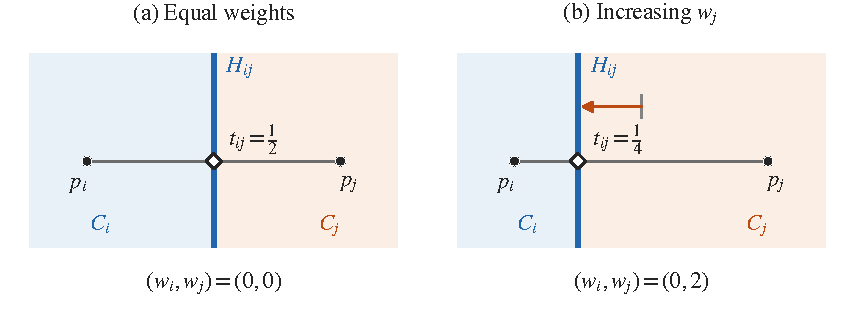
\includegraphics[width=\linewidth]{figures/figure_02_separators.pdf}
\caption{Two fixed sites with equal and unequal weights. (a) Equal weights give the ordinary Voronoi boundary at the midpoint. (b) Increasing $w_j$ moves the boundary toward $p_i$ and enlarges the cell of $p_j$. Both panels use the same sites and scale. With only two sites, the entire pairwise separator is a shared boundary.}
\label{fig:two-site-separators}
\end{figure}

Choosing parameters from observations gives an inverse problem whose form depends on what is known about the desired partition. Duan et al.\ recover site positions and weights from a supplied Laguerre tessellation \cite{Duan2014}. Spettl et al.\ fit a Laguerre approximation to segmented tomographic images, minimizing squared distances from interface samples to pairwise separating planes while varying both site positions and radii \cite{Spettl2016}. Bourne, Pearce and Roper instead recover or fit tessellations from cell volumes and centroids using optimal transport \cite{BournePearceRoper2025}.

Other constructions prescribe which cells must meet. Alexa computes weights at fixed sites, when feasible, so that selected cells have a common intersection, producing meshes that contain prescribed edges or triangles \cite{Alexa2020}. Related methods permit additional sites and subdivisions of the prescribed elements \cite{Bogiokas2025}. In these constructions, the required intersections are part of the input; they need not follow from a fit to measured boundary locations.

We study a setting in which the sites are fixed and the inputs are numerical dividing positions for selected pairs. The positions may be inferred from interface samples or predicted independently, without a supplied global partition. For example, atomic density profiles can predict a dividing position along the line through two nuclei without assigning the rest of space to either atom. The nuclear coordinates specify the molecular geometry, so retaining them is part of the modeling task. We seek one set of site weights that reconciles these local positions. For a given pair, the fixed sites determine the orientation of its separator; one coordinate on the full line through them specifies its position and hence a desired weight difference. Observations may be missing, repeated or noisy.

One weight participates in every observation involving its site, so independently chosen separator positions can impose conflicting requirements. We represent sites by graph vertices and observations by edges. Around a closed chain of observations, the signed weight differences must sum to zero. If compatible observations connect all sites, they determine the weights up to a common shift that leaves the diagram unchanged. When observations conflict, weighted least squares reconciles them through a classical graph-Laplacian problem \cite{Jiang2011}. For interface samples, this quadratic fit is also the fixed-site form of Spettl et al.'s interface discrepancy, with their squared radii identified as weights \cite{Spettl2016}.

Agreement with the pairwise positions does not ensure that the corresponding cells share a face. On a pairwise separator, the two power distances are equal; yet at every point some other site may have a smaller power distance. Even if a common face exists, it may lie away from the line through the pair. We therefore check both the realized faces and whether they contain the separator's intersection with the site line. Fitting the separator positions and assessing their geometric realization are separate steps.

We develop compatibility and identifiability conditions for these observations, together with fitting formulations for noisy data and hard bounds on separator positions. When the line--plane intersection lies inside a face, its distance to the face boundary, measured within the separator plane, defines \emph{centered clearance}. For fixed, unconstrained least-squares problems in finite nonperiodic configurations, perturbation bounds connect changes in the observations to stability of the local test. A computational workflow combines fitting, diagram construction and face checking, including periodic systems, and is implemented in \texttt{pyvoro2} \cite{Pyvoro2_063}.

Synthetic experiments test recovery from exact compatible data and the effects of missing observations, noise and model mismatch. An application to 100 molecules compares predictions from atomic density profiles, their fitted separators and the resulting pair relations with a reference derived from the Quantum Theory of Atoms in Molecules (QTAIM) \cite{Bader1990}. The experiments show that closer agreement with imposed local targets need not improve agreement with an independent reference. In the molecular tests, clearance helps distinguish reference contacts among nonbonded faces that pass the local test. These comparisons concern separator positions and pair relations; complete atomic basins are not reconstructed \cite{PowerfitArchive2026}.

Sections~2--4 develop the observation model, graph fitting and geometric assessment. Section~5 describes the computational workflow. Sections~6 and~7 present the synthetic experiments and molecular application, followed by discussion and conclusions in Sections~8 and~9. The appendices contain supporting arguments, geometric qualifications, and implementation and experimental protocols.

\Needspace{10\baselineskip}
\section{Pairwise separator observations}

We now express each observed or predicted dividing position as a target difference of site weights. For distinct fixed sites $p_1,\ldots,p_n\in\mathbb R^d$, let $w_1,\ldots,w_n$ be real weights with squared-length units. We use the power-distance convention introduced above \cite{Aurenhammer1987}:
\begin{equation}
\pi_i(x)=\|x-p_i\|^2-w_i.
\end{equation}
For an ordered pair $i\ne j$, let $H_{ij}$ be the pairwise separator defined by $\pi_i(x)=\pi_j(x)$.

\begin{samepage}
Set $\delta_{ij}=p_j-p_i$ and $d_{ij}=\|\delta_{ij}\|>0$. The full affine line through the two sites is their \emph{connector line}. Its intersection with $H_{ij}$ is $x=p_i+t_{ij}(w)\delta_{ij}$, where coordinates $0$ and $1$ correspond to $p_i$ and $p_j$. Equating the two power distances gives
\begin{equation*}
 t_{ij}(w)^2d_{ij}^2-w_i=[1-t_{ij}(w)]^2d_{ij}^2-w_j,
\end{equation*}
and hence
\begin{equation}
\boxed{t_{ij}(w)=\frac12+\frac{w_i-w_j}{2d_{ij}^2}.}
\label{eq:pair-coordinate}
\end{equation}
\end{samepage}
The coordinate is defined on the full connector line and need not lie in $[0,1]$.

An observed or predicted coordinate $t_{ij}^{\mathrm{obs}}$ gives the target difference
\begin{equation}
 z_{ij}=(2t_{ij}^{\mathrm{obs}}-1)d_{ij}^2.
 \label{eq:target-difference}
\end{equation}
Matching this position requires $w_i-w_j=z_{ij}$; the individual weights remain undetermined. For the displaced separator in Figure~\ref{fig:two-site-separators}, take $p_i=(0,0)$ and $p_j=(2,0)$. Its location $x_1=1/2$ gives $t_{ij}^{\mathrm{obs}}=1/4$ and $z_{ij}=-2$, consistent with the displayed weights $(w_i,w_j)=(0,2)$.

Other forms of data lead to the same target difference. A signed distance $\ell_{ij}^{\mathrm{obs}}$ measured from $p_i$ toward $p_j$ gives $t_{ij}^{\mathrm{obs}}=\ell_{ij}^{\mathrm{obs}}/d_{ij}$. A supplied point $x_{ij}^{\mathrm{obs}}\in\mathbb R^d$ gives the coordinate by orthogonal projection onto the connector:
\begin{equation}
 t_{ij}^{\mathrm{obs}}=\frac{(x_{ij}^{\mathrm{obs}}-p_i)\cdot\delta_{ij}}{d_{ij}^2}.
\end{equation}
The associated target plane is perpendicular to the connector and passes through $x_{ij}^{\mathrm{obs}}$. Only the longitudinal component enters Eq.~\eqref{eq:target-difference}; the point's transverse displacement has no effect on the target.

Several measurements or predictions may refer to the same pair and yield different targets. We therefore index \emph{observations}, rather than just pairs, by $r$. Let $(i_r,j_r)$ denote the ordered site pair and $y_r$ the supplied normalized coordinate or signed distance. Let $\varepsilon_r$ denote the discrepancy between $y_r$ and the prediction for a candidate weight vector, in the units of $y_r$. Both conventions have the affine form
\begin{align}
 y_r&=\beta_r+\alpha_r(w_{i_r}-w_{j_r})+\varepsilon_r,\label{eq:observation-model}\\
 (\beta_r,\alpha_r)&=
 \begin{cases}
 (\frac12,\frac{1}{2d_r^2}), &\text{normalized coordinate},\\[4pt]
 (\frac{d_r}{2},\frac{1}{2d_r}), &\text{signed distance},
 \end{cases}
\end{align}
where $d_r=\|p_{j_r}-p_{i_r}\|>0$ in the nonperiodic case. Each observation supplies the target difference $z_r=(y_r-\beta_r)/\alpha_r$.

The same model applies to periodic systems once the selected images are specified. Let $1\le\nu\le d$ and let the columns of $\Lambda\in\mathbb R^{d\times\nu}$ form a linearly independent basis of a fixed translation lattice. Observation $r$ specifies a shift $s_r\in\mathbb Z^\nu$, selecting $p_{j_r}^{(s_r)}=p_{j_r}+\Lambda s_r$ relative to $p_{i_r}$. It replaces $p_{j_r}$ in the connector, so $d_r=\|p_{j_r}^{(s_r)}-p_{i_r}\|$, while retaining the base-site weight $w_{j_r}$.

We require $i_r\ne j_r$ and $d_r>0$, excluding observations between images of the same base site and coincident selected endpoints. Different shifts label distinct geometric observations even when they constrain the same two weight variables. Coincident unselected images are discussed in~\ref{app:geometry-periodic}.

The next section determines when these target differences can be satisfied simultaneously and how to reconcile them otherwise. Whether the fitted pairwise planes contribute actual shared cell faces is a separate geometric question, treated in Section~4.

\section{Compatibility and inverse fitting on observation graphs}

\subsection{Observation graph, compatibility, and identifiability}

For a single set of weights to reproduce all observed pairwise separators, their implied weight differences must be mutually compatible.

\begin{samepage}
Consider, for example, three sites with target differences
\begin{equation}
w_1-w_2=0,\qquad w_2-w_3=0,\qquad w_1-w_3=1.
\label{eq:incompatible-triangle}
\end{equation}
The first two equations imply $w_1=w_3$, contradicting the third. Thus, no weight vector can satisfy all three observations simultaneously.
\end{samepage}

We represent the observations by a graph whose vertices are the sites and whose oriented edges $r:i_r\to j_r$ carry the target differences $z_r$. Repeated observations of the same pair correspond to parallel edges. In periodic systems, the vertices remain the base sites: observations with different image shifts are distinct edges even when they involve the same two weight variables. Let $B\in\mathbb R^{n\times m}$ be the incidence matrix of this graph, where $m$ is the number of observations and column $r$ is $e_{i_r}-e_{j_r}$, with $e_i$ the $i$th standard basis vector. The exact fitting conditions become
\begin{equation}
B^Tw=z.
\label{eq:exact-incidence}
\end{equation}
This is a standard graph-potential representation of pairwise differences \cite{Jiang2011}.

Figure~\ref{fig:incompatible-cycle} shows the signed cycle sum for this example. For any weight vector, the corresponding sum of differences must vanish by telescoping. This gives the general compatibility condition below.

\begin{figure}[tbp]
\centering
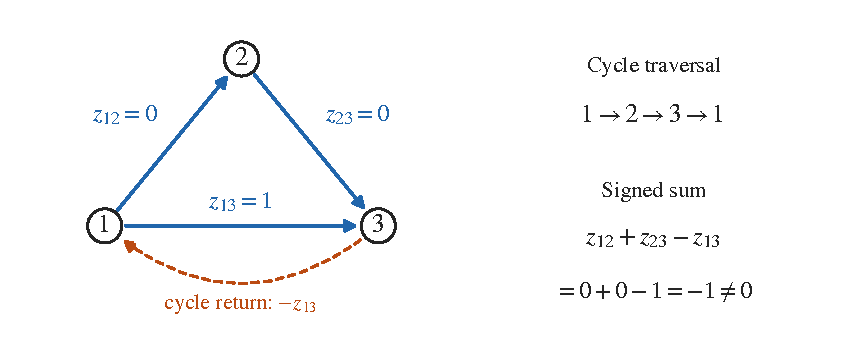
\includegraphics[width=\linewidth]{figures/figure_03_cycle.pdf}
\caption{An abstract observation graph, with no geometric meaning assigned to the vertex positions. Solid arrows orient the three observations in Eq.~\eqref{eq:incompatible-triangle}. The cycle $1\to2\to3\to1$ traverses the $1\to3$ observation backwards (dashed return), giving the contribution $-z_{13}$. This is a signed traversal of the underlying undirected graph, not a fourth observation. Its nonzero sum prevents any single weight vector from reproducing all three targets.}
\label{fig:incompatible-cycle}
\end{figure}
\FloatBarrier

\begin{proposition}[Cycle compatibility]
\label{prop:cycle-compatibility}
Let $G$ be the observation multigraph with incidence matrix $B$ and target differences $z\in\mathbb R^m$. A weight vector $w\in\mathbb R^n$ satisfying $B^Tw=z$ exists if and only if the signed sum of target differences vanishes around every cycle of the underlying undirected multigraph:
\begin{equation}
\sum_{r\in C}\operatorname{sgn}_C(r)\,z_r=0.
\label{eq:cycle-sum}
\end{equation}
Here $\operatorname{sgn}_C(r)=+1$ when the cycle traverses edge $r$ in its assigned orientation and $-1$ otherwise. Cycles formed by two parallel edges are included.
\end{proposition}

\begin{proof}
If $B^Tw=z$, each target difference equals the difference of its endpoint weights. Summing these differences around any cycle gives zero by telescoping.

Conversely, choose a spanning forest of $G$ and assign an arbitrary weight to one root in each connected component. The observations on the forest edges uniquely determine the remaining weights within each component. Every edge outside the forest closes a cycle with the corresponding forest path. By the assumed cycle condition, its target difference agrees with the difference already determined along that path. Thus, all observations are satisfied.
\end{proof}

In particular, repeated observations of the same pair must have identical targets after accounting for their orientations. The construction also leaves one arbitrary additive constant per connected component, leading to the identifiability question considered next.

\begin{corollary}[Identifiability]
\label{cor:observation-identifiability}
Let the observation graph $G$ have $c$ connected components $C_1,\ldots,C_c$, including isolated vertices. If the observations are compatible and $w^\star$ is one solution of $B^Tw=z$, then every solution has the form
\begin{equation}
w=w^\star+\sum_{a=1}^{c}\gamma_a\mathbf{1}_{C_a},
\qquad \gamma_a\in\mathbb R,
\label{eq:component-gauge}
\end{equation}
where $\mathbf{1}_{C_a}$ is the indicator vector of component $C_a$. Consequently, the difference $w_i-w_j$ is uniquely determined by the observations if and only if sites $i$ and $j$ belong to the same connected component. Equivalently, $\operatorname{rank}(B)=n-c$.
\end{corollary}

\begin{proof}
The difference between any two solutions belongs to $\ker B^T$, so it must be constant across every observed edge, and hence within each connected component. Conversely, adding an arbitrary constant to the weights in any component leaves all observed differences unchanged.
\end{proof}

This ambiguity in the observations must be distinguished from a symmetry of the power diagram itself. Adding the same constant to every site weight leaves all power-distance comparisons unchanged and therefore preserves the complete diagram. In contrast, shifting the weights of disconnected observation components independently can change the competition between their cells. Thus, fixing one additive constant per component selects a particular solution, but may also select a particular geometry among several that are equally consistent with the observations.

\subsection{Fitting inconsistent observations}

When the cycle-compatibility conditions of Section~3.1 are violated, no weight vector can satisfy all observations exactly. We therefore seek weights that minimize the discrepancies between the observed separator positions and their predictions under the power model.

For each observation $r$, let $\lambda_r>0$ be the weight assigned to its squared residual in the original measurement units. Using the affine observation model from Section~2, we minimize
\begin{equation}
\mathcal E(w)=\frac12\sum_{r=1}^{m}
\lambda_r\left[
y_r-\beta_r-\alpha_r(w_{i_r}-w_{j_r})
\right]^2.
\label{eq:measured-least-squares}
\end{equation}
With the target differences $z_r=(y_r-\beta_r)/\alpha_r$, the same objective becomes
\begin{equation}
\boxed{
\mathcal E(w)=\frac12\sum_{r=1}^{m}
\rho_r\left[(w_{i_r}-w_{j_r})-z_r\right]^2,
\qquad \rho_r=\lambda_r\alpha_r^2.
}
\label{eq:difference-least-squares}
\end{equation}
This transformation preserves the objective but changes the weights assigned to individual residuals. Since $\alpha_r$ depends on the observation type and connector length, equal weights in the original measurement units do not generally imply equal weights on the inferred differences.

Let $R=\operatorname{diag}(\rho_1,\ldots,\rho_m)$. Using the incidence matrix $B$ from Section~3.1, we can write the objective as
\begin{equation}
\mathcal E(w)=\frac12(B^Tw-z)^TR(B^Tw-z).
\label{eq:matrix-least-squares}
\end{equation}
Differentiation gives
\begin{equation}
\nabla\mathcal E(w)=BR(B^Tw-z).
\end{equation}
Since the objective is convex, its minimizers are characterized by the normal equations
\begin{equation}
\boxed{Lw=BRz,\qquad L=BRB^T.}
\label{eq:laplacian-normal}
\end{equation}

Here $L$ is the weighted graph Laplacian, as in classical graph-potential least squares \cite{Jiang2011}. For any $v\in\mathbb R^n$,
\begin{equation}
v^TLv=\sum_{r=1}^{m}\rho_r(v_{i_r}-v_{j_r})^2\ge 0.
\end{equation}
Since all $\rho_r>0$, this also shows that $\ker L=\ker B^T$, the space of vectors that are constant on each connected component of the observation graph. Moreover, $BRz$ is orthogonal to this nullspace and hence belongs to the range of $L$. Thus, the normal equations have a solution for every $z$, even when the target differences are incompatible. Their solutions differ only by componentwise additive constants. Fixing these unobservable constants selects one representative; we call this a \emph{gauge convention}.

For the inconsistent three-site example in Fig.~\ref{fig:incompatible-cycle}, with equal fitting weights $\rho_r$ and the gauge $w_3=0$, the least-squares solution is
\begin{equation}
(w_1,w_2,w_3)=\left(\frac23,\frac13,0\right).
\end{equation}
The residuals $B^Tw-z=(1/3,\,1/3,\,-1/3)$ follow the order of the three observations. Each therefore has magnitude $1/3$: the fit balances the conflicting observations rather than selecting one to discard.

For fixed generator positions, this quadratic structure also follows from
the interface discrepancy of Spettl et al.\ \cite{Spettl2016}.
For a point $x$ assigned to pair $i,j$, identifying squared generator
radii with the weights gives
\[
\begin{aligned}
z_{ij}(x)
 &=2(p_j-p_i)\cdot x+\|p_i\|^2-\|p_j\|^2,\\
\operatorname{dist}\bigl(x,H_{ij}(w)\bigr)^2
 &=\frac{[(w_i-w_j)-z_{ij}(x)]^2}{4d_{ij}^2}.
\end{aligned}
\]
Summing these terms yields a weighted difference fit of the form above,
up to an overall positive normalization. Multiple points assigned to
one pair can be grouped into their mean target with the corresponding
total fitting weight, plus an additive constant independent of $w$.
This reduction assumes fixed generator positions; the published method
also optimizes those positions.
The additive constant records the spread of the projected sample positions.
Replacing the samples by their mean preserves the optimal weights, but
agreement with that mean need not imply a small error over the sampled
interface. Thus, data sufficient to determine the weights need not suffice
to assess the approximation of an entire boundary.

The quadratic loss is not essential to the observation model. When large residuals should have less influence, the squared penalties can be replaced by convex losses such as the Huber loss, which is quadratic near zero and linear beyond a residual threshold \cite{Huber1964}. The resulting fixed-observation problem remains convex, although its minimizer is generally no longer obtained from a linear Laplacian system.

\subsection{Hard separator constraints}

Some separator requirements must be satisfied exactly rather than treated as approximate targets. We allow a separate set $\mathcal I_{\mathrm H}$ of hard restrictions, which may involve site pairs absent from the $m$ observations used for fitting. For each $h\in\mathcal I_{\mathrm H}$, let $(i_h,j_h)$ be the ordered site pair, and let $[\underline y_h,\overline y_h]$ specify an admissible interval in one of the measurement conventions of Section~2. With the corresponding coefficients $\beta_h$ and $\alpha_h>0$, the restriction reads
\begin{equation}
\underline y_h\le
\beta_h+\alpha_h(w_{i_h}-w_{j_h})
\le\overline y_h.
\label{eq:hard-measurement-interval}
\end{equation}
This is equivalent to the bounds
\begin{equation}
\boxed{\ell_h\le w_{i_h}-w_{j_h}\le u_h,}
\label{eq:hard-weight-interval}
\end{equation}
where
\begin{equation}
\ell_h=\frac{\underline y_h-\beta_h}{\alpha_h},
\qquad
u_h=\frac{\overline y_h-\beta_h}{\alpha_h}.
\end{equation}
An exact separator requirement is the special case $\ell_h=u_h$. Unlike residuals in the least-squares objective, these restrictions must be satisfied by the fitted weights.

Their joint feasibility is described by a directed graph of \emph{difference constraints}: each inequality $w_v\le w_u+c_{uv}$ is represented by an arc $u\to v$ with cost $c_{uv}$. This constraint graph differs from the observation multigraph used for fitting. The standard negative-cycle criterion \cite[Sec.~24.4]{Cormen2009} takes the following form in our sign convention.

\begin{proposition}[Feasibility of difference constraints]
\label{prop:hard-feasibility}
Consider a finite collection of restrictions
\begin{equation}
\ell_h\le w_{i_h}-w_{j_h}\le u_h,
\qquad h\in\mathcal I_{\mathrm H},
\end{equation}
with finite real bounds $\ell_h,u_h$. Construct a directed weighted multigraph on the sites by adding, for each restriction $h$, an arc $j_h\to i_h$ with cost $u_h$ and an arc $i_h\to j_h$ with cost $-\ell_h$.

There exists a weight vector satisfying all restrictions if and only if this graph contains no directed cycle with negative total cost.
\end{proposition}

\begin{proof}
Summing the inequalities represented by arcs around any directed cycle cancels the site weights, so every cycle must have nonnegative total cost.

Conversely, suppose there are no negative directed cycles. Add an auxiliary source connected to every vertex by a zero-cost arc, and let $d(v)$ be the shortest-path distance from this source to vertex $v$. These distances are finite and satisfy
\begin{equation}
d(v)\le d(u)+c_{uv}
\end{equation}
for every arc $u\to v$. Therefore, setting $w_v=d(v)$ satisfies every difference constraint.
\end{proof}

The criterion can be checked using standard shortest-path algorithms, such as Bellman--Ford \cite{Bellman1958}. A negative cycle certifies infeasibility of the prescribed restrictions, independently of any least-squares objective.

When hard restrictions are feasible, they can be imposed on the least-squares fit. Let
\begin{equation}
\mathcal H=\left\{w\in\mathbb R^n:
\ell_h\le w_{i_h}-w_{j_h}\le u_h
\text{ for all }h\in\mathcal I_{\mathrm H}\right\}.
\label{eq:hard-feasible-set}
\end{equation}
The resulting optimization problem is
\begin{equation}
\boxed{
\min_{w\in\mathcal H}
\frac12(B^Tw-z)^TR(B^Tw-z).
}
\label{eq:hard-constrained-fit}
\end{equation}
This is a convex quadratic program. Whenever $\mathcal H$ is nonempty, the minimum is attained, as proved in~\ref{app:constrained-attainment}. Any two minimizers differ by constants on the connected components of the observation graph, but only shifts that preserve $\mathcal H$ remain admissible. In particular, hard restrictions connecting different components may constrain their relative offsets, so independently fixing one constant per component is no longer an arbitrary gauge choice. A common shift of all site weights remains free.

Algebraic compatibility, optimal fitting, and feasibility of hard restrictions do not guarantee that the corresponding site pairs share actual faces in the resulting power diagram. We address geometric realization in the next section.

\section{Geometric realization and local diagnostics}
\label{sec:geometric-realization}

% Audited foundation; deterministic figure integrated 2026-10-30.

\subsection{Pairwise separators and realized faces}
\label{subsec:faces}

For a finite nonperiodic configuration, the \emph{power cell} $C_i(w)$ of site $i$ consists of all points at which its power distance is minimal among the sites \cite{Aurenhammer1987}. For two distinct sites $i$ and $j$, we distinguish their \emph{pairwise bisector} $H_{ij}(w)$, where their power distances are equal, from their \emph{common cell intersection} $F_{ij}(w)$, where both sites attain the minimum power distance. Explicitly,
\begin{align}
C_i(w)&=\{x\in\mathbb R^d:\pi_i(x)\le\pi_k(x)
\text{ for all }k\}, \label{eq:power-cell}\\[2pt]
H_{ij}(w)&=\{x\in\mathbb R^d:\pi_i(x)=\pi_j(x)\}, \label{eq:pair-bisector}\\[2pt]
F_{ij}(w)&=C_i(w)\cap C_j(w)\notag\\
&=\{x\in H_{ij}(w):
\pi_i(x)\le\pi_k(x)
\text{ for all }k\ne i,j\}. \label{eq:common-cell-intersection}
\end{align}

While the position of $H_{ij}$ depends only on the weight difference $w_i-w_j$, the existence and extent of $F_{ij}$ depend on the competing sites and their weights. In particular, $F_{ij}$ may be empty even when the pairwise separator is fitted exactly. Moreover, a nonempty intersection need not form a full $(d-1)$-dimensional face: the two cells may meet only in a lower-dimensional set.

Recall that Section~2 describes the position of a pairwise separator by its coordinate along the line through the two sites. For fitted weights, this identifies a particular point on the pairwise bisector,
\begin{equation}
q_{ij}(w)=p_i+t_{ij}(w)(p_j-p_i)\in H_{ij}(w).
\label{eq:connector-point}
\end{equation}
This gives a second geometric question beyond the existence of a shared face: does this particular point belong to the common cell intersection $F_{ij}$? The condition $q_{ij}\in F_{ij}$ is stronger than $F_{ij}\ne\varnothing$, since a shared face may lie elsewhere on the bisector. The following example illustrates both distinctions.

Consider four sites in the plane,
\begin{equation}
p_1=(0,0),\quad p_2=(2,0),\quad
p_3=(1,1),\quad p_4=(1,-1),
\label{eq:four-sites}
\end{equation}
with $w_1=w_2=0$. The pairwise bisector of sites 1 and 2 is always $H_{12}=\{(1,y):y\in\mathbb R\}$, and its intersection with the line through the two sites is $q_{12}=(1,0)$, regardless of the weights assigned to sites 3 and 4. The conditions imposed by these competing sites give
\begin{equation}
F_{12}=\left\{(1,y):
\frac{w_4}{2}\le y\le-\frac{w_3}{2}\right\}.
\label{eq:four-site-face}
\end{equation}

Figure~\ref{fig:three-face-cases} shows how changing only the competing weights makes the shared face disappear, moves it away from the connector, or places the connector point inside it.

\begin{figure}[!tb]
\centering
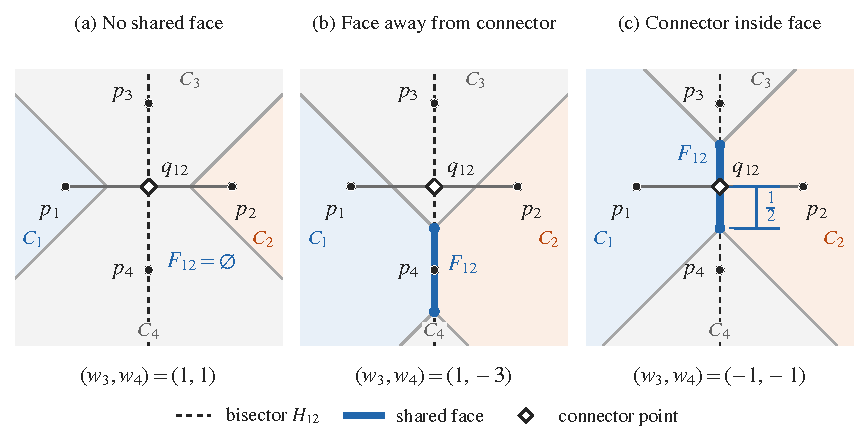
\includegraphics[width=\linewidth]{figures/figure_04_realization.pdf}
\caption{Three outcomes for the fixed sites in Eq.~\eqref{eq:four-sites}, with $w_1=w_2=0$. The dashed bisector $H_{12}$ and diamond $q_{12}$ stay fixed. Shading distinguishes the power cells; the blue segment shows $F_{12}$ when it is nonempty. (a) $F_{12}=\varnothing$. (b) $F_{12}=\{1\}\times[-3/2,-1/2]$, away from $q_{12}$. (c) $F_{12}=\{1\}\times[-1/2,1/2]$, with $q_{12}$ strictly inside; the bracket measures the distance $1/2$ to an endpoint. Site markers need not lie in their own cells: in (b), $p_4\in F_{12}$ but $p_4\notin C_4$. All panels use the same scale and drawing window; the cells are defined in the full plane.}
\label{fig:three-face-cases}
\end{figure}

Since $F_{ij}$ lies in the $(d-1)$-dimensional hyperplane $H_{ij}$, it contains a full $(d-1)$-dimensional portion precisely when
\begin{equation}
\boxed{\operatorname{int}_{H_{ij}}F_{ij}\ne\varnothing,}
\label{eq:full-dimensional-face}
\end{equation}
where $\operatorname{int}_{H_{ij}}$ denotes interior within the entire bisector hyperplane. Equivalently, $F_{ij}$ must contain a nonempty open ball measured within $H_{ij}$. When both power cells are themselves full-dimensional, such an intersection is a shared facet of the two cells.

The distinction is visible in the four-site example. With $(w_3,w_4)=(1,-1)$, the bounds defining $F_{12}$ meet at $y=-1/2$, leaving only the point $(1,-1/2)$. The cells intersect, but they do not share an edge.

Further degeneracies are discussed in~\ref{app:geometry-degeneracy}. We next test connector membership using power-distance comparisons.

\subsection{Connector visibility}
\label{subsec:connector-visibility}

The fitted separator coordinate fixes $q_{ij}$, so testing $q_{ij}\in F_{ij}$ checks geometric support at that location without searching for another witness on the bisector.

To perform this test, we compare the power distances of the pair with those of the competing sites at $q_{ij}$. For each $k\notin\{i,j\}$, define the \emph{competitor gap}
\begin{equation}
g_{ijk}(w)=\pi_k(q_{ij}(w))-\pi_i(q_{ij}(w)).
\label{eq:competitor-gap}
\end{equation}
Since $\pi_i(q_{ij})=\pi_j(q_{ij})$, the point belongs to both power cells exactly when no competitor has a smaller power distance. Thus,
\begin{equation}
\boxed{q_{ij}(w)\in F_{ij}(w)
\quad\Longleftrightarrow\quad
g_{ijk}(w)\ge0
\quad\text{for all }k\notin\{i,j\}.}
\label{eq:weak-connector-visibility}
\end{equation}

We refer to this as \emph{weak connector visibility}. Strict positivity of every competitor gap provides a stronger certificate: for a finite configuration, the inequalities remain satisfied in a neighborhood of $q_{ij}$ within the bisector. Consequently,
\begin{equation}
g_{ijk}(w)>0\quad\text{for all }k\notin\{i,j\}
\quad\Longrightarrow\quad
q_{ij}(w)\in\operatorname{int}_{H_{ij}}F_{ij}(w).
\label{eq:strict-connector-visibility}
\end{equation}
Strict competitor inequalities also persist in a small ambient neighborhood of $q_{ij}$. On opposite sides of the bisector near that point, sites $i$ and $j$, respectively, are the unique power minimizers. Thus strict visibility certifies a genuine local facet between two full-dimensional cells.

When all site weights are equal, $q_{ij}$ is the midpoint, and strict positivity of the gaps means that every other site lies outside the closed ball with diameter $p_ip_j$. This is the strict form of the classical \emph{Gabriel} edge condition. Its weighted counterpart uses the full affine connector line, so the witness may lie outside the site segment \cite[Sec.~2]{Alexa2020}. The all-strict test above is therefore a weighted Gabriel edge certificate. We use \emph{weak connector visibility} separately for the non-strict condition $q_{ij}\in F_{ij}$, which permits boundary contacts and persistent ties and does not by itself certify a genuine facet; see~\ref{app:geometry-degeneracy}.

The competitor gaps can be expressed directly in terms of the fitted weights. Writing $\delta_{ij}=p_j-p_i$ and $q_{ij}=p_i+t_{ij}\delta_{ij}$, expansion of the squared distances gives
\begin{equation}
g_{ijk}(w)=
\|p_k-p_i\|^2
-2t_{ij}(w)\,\delta_{ij}\cdot(p_k-p_i)
+w_i-w_k.
\label{eq:gap-affine-formula}
\end{equation}
Since $t_{ij}(w)$ is affine in $w_i-w_j$, each competitor gap is an affine function of the site weights for fixed site positions. It is also invariant under adding a common constant to all weights.

For a pair $i,j$, we summarize the competitor inequalities by the \emph{minimum signed gap}
\begin{equation}
\boxed{\sigma_{ij}(w)=\min_{k\notin\{i,j\}}g_{ijk}(w).}
\label{eq:minimum-signed-gap}
\end{equation}
When there are no competing sites, we set $\sigma_{ij}=+\infty$. Otherwise, $\sigma_{ij}$ is a continuous, piecewise-affine function of the weights. The weak connector-visibility condition is equivalent to $\sigma_{ij}\ge0$, while $\sigma_{ij}>0$ guarantees strict visibility and a full-dimensional shared face near $q_{ij}$. A negative value only establishes that the selected connector point is not on the shared face; it does not exclude a face elsewhere on the bisector.

In Fig.~\ref{fig:three-face-cases}(a--c), the values of $\sigma_{12}$ are respectively $-1$, $-1$, and $+1$. The same negative score occurs both when the face is absent and when it lies away from the connector.

\subsection{Connector-centered clearance}
\label{subsec:connector-clearance}

A strictly positive minimum signed gap $\sigma_{ij}$ places the connector point in the interior of $F_{ij}$ within the bisector. The gap has units of squared length, however, and does not directly describe the geometric extent of this interior neighborhood.

When $q_{ij}\in F_{ij}$, we define the \emph{connector-centered clearance} $c_{ij}$ as the supremum of radii $r\ge0$ for which the in-bisector Euclidean ball
\begin{equation}
B_{H_{ij}}(q_{ij},r)
=\{q_{ij}+u:
u\cdot\delta_{ij}=0,\ \|u\|\le r\}
\label{eq:bisector-ball}
\end{equation}
is contained in $F_{ij}$. This is a ball of dimension $d-1$, with the Euclidean metric inherited from $\mathbb R^d$, and its center is fixed at $q_{ij}$.

Let $e_{ijk}$ be the component of $p_k-p_i$ perpendicular to the site connector:
\begin{equation}
e_{ijk}
=(p_k-p_i)
-\frac{(p_k-p_i)\cdot\delta_{ij}}
{\|\delta_{ij}\|^2}\delta_{ij}.
\label{eq:projected-competitor}
\end{equation}
For any displacement $u$ within the bisector, the difference of power distances becomes
\begin{equation}
\pi_k(q_{ij}+u)-\pi_i(q_{ij}+u)
=g_{ijk}-2e_{ijk}\cdot u.
\label{eq:power-gap-displacement}
\end{equation}

The smallest value of this expression over $B_{H_{ij}}(q_{ij},r)$ is $g_{ijk}-2r\|e_{ijk}\|$. Thus, the entire ball is contained in the common cell intersection exactly when
\begin{equation}
2r\|e_{ijk}\|\le g_{ijk}
\qquad\text{for every competitor }k.
\label{eq:clearance-inequalities}
\end{equation}
It follows that, for $\sigma_{ij}>0$,
\begin{equation}
\boxed{
c_{ij}(w)=
\min_{\substack{k\notin\{i,j\}\\\|e_{ijk}\|>0}}
\frac{g_{ijk}(w)}{2\|e_{ijk}\|}.
}
\label{eq:connector-clearance}
\end{equation}
The minimum over an empty set is $+\infty$, corresponding to $F_{ij}=H_{ij}$. Under strict visibility, competitors with $e_{ijk}=0$ impose no restriction on motion within the bisector.

In Fig.~\ref{fig:three-face-cases}(c), both competitor gaps and both projected distances equal $1$. Hence $c_{12}=1/2$, the marked distance from $q_{12}$ to an endpoint of the shared edge.

% PRO-REVIEW: Is the exterior-distance discussion sufficiently motivated
% and economical, given the planned implementation-level usage?
The formula should not be extended to negative gaps by simply allowing a negative clearance. When $\sigma_{ij}<0$, the connector point lies outside $F_{ij}$, so no centered ball, not even one of radius zero, is contained in the common cell intersection. Moreover, a negative value of the expression above describes a violation of an individual competitor inequality, whereas the distance to the actual face depends on satisfying all inequalities simultaneously. The face may even be empty.

For a nonempty face, the appropriate exterior measure is instead the Euclidean distance from $q_{ij}$ to $F_{ij}$, measured within the bisector. In~\ref{app:geometry-exterior}, we derive its computation as a convex projection problem and illustrate why a negative extension of Eq.~\eqref{eq:connector-clearance} does not generally give this distance. The zero-gap clearance formula is treated in~\ref{app:geometry-exterior}; persistent ties are discussed in~\ref{app:geometry-degeneracy}. 

\subsection{Stability of geometric support}
\label{subsec:geometric-stability}

The diagnostics above refer to a particular set of fitted weights. Errors in separator observations can perturb these weights, so we ask when the resulting connector-visibility classification remains stable.

We first consider a fixed finite, nonperiodic site configuration. For a pair $i,j$ and competitor $k$, define the dimensionless coefficient
\begin{equation}
\theta_{ijk}
=\frac{(p_k-p_i)\cdot(p_j-p_i)}
{\|p_j-p_i\|^2}.
\label{eq:stability-theta}
\end{equation}
This is the coordinate of the orthogonal projection of $p_k$ onto the affine line through $p_i,p_j$. From the affine expression for the competitor gap in Section~4.2, a weight perturbation $\Delta w$ gives the exact identity
\begin{equation}
g_{ijk}(w+\Delta w)-g_{ijk}(w)
=(1-\theta_{ijk})\Delta w_i
+\theta_{ijk}\Delta w_j-\Delta w_k.
\label{eq:gap-weight-perturbation}
\end{equation}
Consequently, defining
\begin{equation}
K_{ij}=
\max_{k\notin\{i,j\}}
\left(
|1-\theta_{ijk}|+|\theta_{ijk}|+1
\right),
\label{eq:gap-lipschitz-constant}
\end{equation}
we obtain
\begin{equation}
\boxed{
|\sigma_{ij}(w+\Delta w)-\sigma_{ij}(w)|
\le K_{ij}\|\Delta w\|_\infty.
}
\label{eq:gap-lipschitz-bound}
\end{equation}
Here the competitor set is assumed nonempty. The bound follows because each competitor gap satisfies the corresponding estimate and taking the minimum cannot increase the largest absolute change.

In particular, if $\sigma_{ij}(w)>0$ and
\begin{equation}
K_{ij}\|\Delta w\|_\infty<\sigma_{ij}(w),
\label{eq:strict-stability-condition}
\end{equation}
then $\sigma_{ij}(w+\Delta w)>0$. Thus, the pair retains strict connector visibility, and its common face remains full-dimensional near the perturbed connector point.

The same argument preserves a negative sign when the perturbation bound is smaller than $|\sigma_{ij}(w)|$. This only certifies that the connector point remains outside the shared face; it does not establish that the face is absent. At zero margin, the bound provides no sign-preservation guarantee.

Because the competitor gaps are invariant under a common shift of all site weights, the perturbation bound may also be expressed using the smallest infinity norm after subtracting such a shift. The result concerns the connector-visibility status of the selected pair, not the topology of the entire power diagram.

The preceding bound concerns perturbations of the site weights. To relate it to errors in the observed separators, consider the unconstrained quadratic fit of Section~3 with a fixed observation graph and fixed positive fitting weights.

Let $z^\star$ be a reference vector of target differences, not necessarily compatible, and let $\widehat z=z^\star+\eta$ be a perturbed observation vector. Denote their least-squares solutions by $w^\star$ and $\widehat w$, respectively, using the same fixed linear convention for the undetermined component offsets. For this fixed fitting problem, the solution depends linearly on the targets. Writing this dependence as $w=Gz$, we obtain
\begin{equation}
\widehat w-w^\star=G\eta.
\label{eq:weight-response}
\end{equation}
Combining this identity with the geometric perturbation bound gives
\begin{equation}
\boxed{
|\sigma_{ij}(\widehat w)-\sigma_{ij}(w^\star)|
\le K_{ij}\|G\eta\|_\infty
\le K_{ij}\|G\|_{\infty\to\infty}\|\eta\|_\infty.
}
\label{eq:observation-to-visibility}
\end{equation}
If the right-hand side is smaller than $|\sigma_{ij}(w^\star)|$, the connector-visibility score keeps its sign.

The conclusion concerns the visibility classification of the \emph{reference least-squares fit}. It does not automatically establish agreement with an independently specified physical weight vector: any difference between that vector and the reference fit must also be accounted for. Moreover, when the observation graph is disconnected, the chosen component offsets affect the geometry, so the comparison requires a consistent convention. The reduced-Laplacian response and error bounds are given in~\ref{app:stability-estimator}; the additional bias when comparing with independent physical reference weights is treated in~\ref{app:stability-reference}.

\paragraph{Clipping and periodic images}
The preceding stability results concern a fixed finite set of sites in an unbounded nonperiodic domain. Clipping and periodicity require additional geometric qualifications.

For a diagram restricted to a convex box $\Omega$, the relevant common cell intersection is
\begin{equation}
F_{ij}^{\Omega}=F_{ij}\cap\Omega.
\label{eq:clipped-face}
\end{equation}
Strictly positive competitor gaps alone do not guarantee that the connector point belongs to this clipped intersection: the point must also lie inside $\Omega$. If $\sigma_{ij}>0$ and $q_{ij}\in\operatorname{int}\Omega$, then a neighborhood of $q_{ij}$ within the bisector belongs to $F_{ij}^{\Omega}$. The corresponding connector-centered clearance is
\begin{equation}
c_{ij}^{\Omega}
=\min\{c_{ij},b_{ij}^{\Omega}\},
\label{eq:clipped-clearance}
\end{equation}
where $b_{ij}^{\Omega}$ is the largest radius of an in-bisector ball centered at $q_{ij}$ and contained in $\Omega$. Intersections confined to the domain boundary require additional care, since an intersection of positive dimension within the bisector need not represent an interface between two full-dimensional cells inside the domain.

For periodic diagrams, the pairwise separator is associated with two selected site images, rather than merely their base-site indices. Every other image can act as a competitor, including other images of either selected base site. The power-gap and clearance constructions remain applicable to these image instances, but their evaluation requires the relevant competing images to be identified correctly. In particular, neither an arbitrary finite image cutoff nor the finite-competitor stability bound derived above is automatically valid for the complete periodic diagram.

See~\ref{app:geometry-clipping} for clipping and~\ref{app:geometry-periodic} for image-aware geometry. Further limitations on periodic perturbation bounds are recorded in~\ref{app:stability-periodic}.

These diagnostics characterize local geometric support of fitted separators. They complement, rather than replace, an explicit examination of the realized power diagram, which forms part of the computational workflow described next.

\section{Computational workflow}
\label{sec:computational-workflow}

A \emph{one-pass calculation} fits all supplied observations and checks which requested faces its diagram realizes (Fig.~\ref{fig:computational-workflow}). When neighbor assignments in the supplied pair list are uncertain, some separator predictions may concern pairs that do not share a face in the fitted diagram. Optional refinement repeats the fit on an active subset of these \emph{candidate observations}. Each observation supplies one row of the fitting problem; the \emph{active mask} records which observations enter the current fit. Requested-image face matches determine which candidates remain active, while every original candidate remains available for matching and possible re-entry. The implementation described here is \texttt{pyvoro2} 0.6.3 \cite{Pyvoro2_063}.

\begin{figure}[!tbp]
\centering
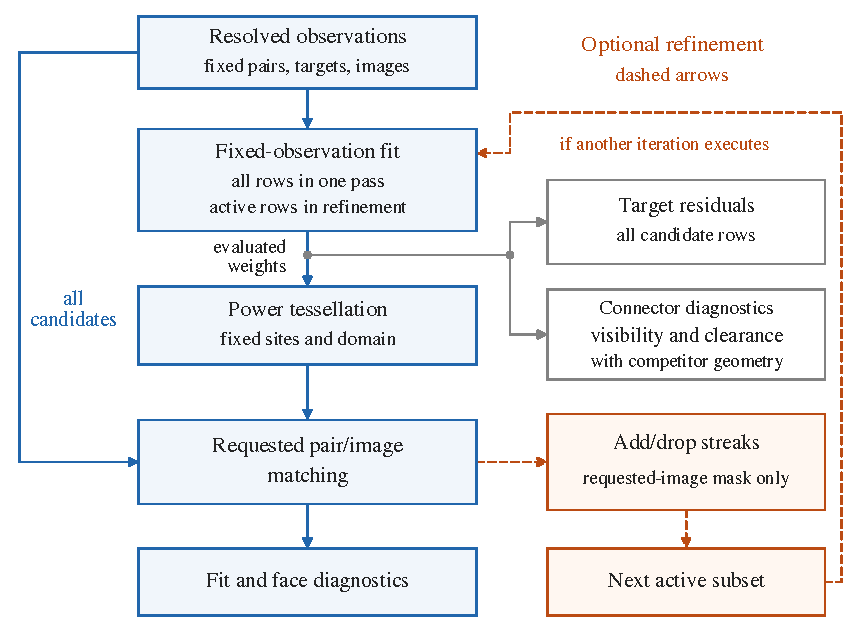
\includegraphics[width=\linewidth]{figures/figure_05_workflow.pdf}
\caption{Data routes for one-pass fitting and optional refinement. Matching receives all resolved candidates; only active rows enter a refined fit. The dashed path updates the active subset using counters of consecutive requested-image realizations or absences. The return to fitting is taken only if another iteration executes. Residuals and connector diagnostics do not drive this update. Sections~\ref{subsec:workflow-active-mask}--\ref{subsec:workflow-output} and~\ref{app:algorithm-implementation} specify alignment, relaxation and finalization.}
\label{fig:computational-workflow}
\end{figure}

\subsection{Resolving observations and fitting a fixed set}
\label{subsec:workflow-fixed-fit}

The inputs are fixed site positions, numerical separator observations, and their assigned fitting weights. A domain is also needed for periodic image resolution or geometric evaluation. Each fitting call uses one measurement convention from Section~2: normalized coordinates or signed distances. An observation retains its ordered pair $(i_r,j_r)$, target $y_r$, and selected image shift $s_r$ in periodic calculations. These choices determine the connector length $d_r$ and affine coefficients $(\alpha_r,\beta_r)$. A supplied periodic shift is part of the observation's identity; when shifts are not supplied, a separate image-selection policy resolves them before fitting. Different shifts for one base pair can label distinct observations while constraining the same weight difference.

For a fixed observation set, the ordinary quadratic fit minimizes the weighted measurement-space residuals of Section~3. With the positive fitting weights assumed there, the implementation solves separately on the observation-graph components using \emph{dense} linear algebra. Since additive component offsets leave the fitted differences unchanged, the solver must choose a representative weight vector on each component. These choices can affect the geometry when several components share a diagram; the version-specific conventions are given in~\ref{app:algorithm-implementation}.

The solver also supports a Huber loss in the original measurement units and hard measurement bounds. A hard restriction applies one common interval or fixed value to every supplied row in those units; this is narrower than the independently indexed restrictions of Section~3.3. Nonquadratic terms or hard restrictions use an iterative solver, and infeasible hard difference bounds are detected by a graph precheck. The Huber threshold is expressed in the selected measurement units, so its equivalent threshold in weight-difference units depends on $\alpha_r$. Predictions are returned as normalized coordinates or signed distances, together with residuals, connectivity warnings, and fitting status. We use the term \emph{fixed-observation fit} to distinguish the rows supplied to the estimator from the faces ultimately realized by the tessellation.

\subsection{Constructing and matching realized faces}
\label{subsec:workflow-realization}

A fitted weight vector $\widehat w$ defines a power diagram but does not guarantee that its observed pairs share actual faces. The three-dimensional backend is Voro++ \cite{Rycroft2009}; two-dimensional calculations use the separately bundled backend exposed by \texttt{pyvoro2.planar} \cite{Pyvoro2_063}. The implementation uses a common shift $C$ such that $\widehat w_i+C\ge0$ and passes radii $r_i=\sqrt{\widehat w_i+C}$. The shift changes none of the power comparisons. Within the chosen two- or three-dimensional domain, the computed cells supply the internal edges or faces that are subsequently matched to the resolved observation rows.

For a periodic observation requesting $(i_r,j_r,s_r)$, the matching step checks that \emph{the specified image shift} occurs among the realized boundaries. The flag \texttt{realized} records a boundary at any shift. An exact requested-image match is marked \texttt{realized\_\allowbreak same\_\allowbreak shift}; if the requested shift is absent but another image is realized, \texttt{realized\_\allowbreak other\_\allowbreak shift} is set. Reversing the pair orientation reverses the shift.

Additional diagnostics flag empty endpoint cells and realized base-site pairs absent from the supplied candidate list, recording the realized shifts of those extra pairs. Boundary length in two dimensions or face area in three dimensions may also be recorded; its image-selection convention is specified in~\ref{app:algorithm-implementation}. Realization here means a boundary reported by the numerical tessellation in the chosen domain.

Requested-image matching examines the actual boundary, whereas the connector tests of Section~4 examine support at a particular point. A realized face can therefore fail connector visibility, as in Fig.~\ref{fig:three-face-cases}(b). Neither property is certified by a small fitting residual.

\subsection{Optional refinement of the observation set}
\label{subsec:workflow-active-mask}

For optional candidate observations, refinement retains a fixed collection of $m$ resolved rows and starts from a Boolean active mask $a^{(0)}\in\{0,1\}^m$, initially all ones unless specified otherwise. At iteration $k$, only rows with $a_r^{(k)}=1$, together with their hard measurement bounds, are supplied to the inner solve. Dropping a row therefore also drops its bound.

For every fit after the first, the weights are aligned component by component with the preceding evaluated weights. Alignment adds a common constant to all weights in each current fitting component, making their mean equal to the preceding mean over the same sites. A relaxation factor $0<\omega\le1$ then blends the aligned fit with the preceding iterate before the diagram is constructed; the initial fit is used without blending. For unregularized fits, alignment preserves the fitting objective while carrying forward component offsets that the pair data do not determine. The optional weight regularizer adds a quadratic penalty for departure from a reference vector. With positive regularization strength, the implementation still aligns the components, which can change the regularized objective; see~\ref{app:algorithm-implementation} for the version-specific regularization and alignment conventions.

The diagram is then evaluated against \emph{every original candidate row}, not only those currently active. For $r=1,\ldots,m$, let
\begin{equation}
v_r^{(k)}=
\begin{cases}
1,&\text{if the requested pair and image shift are realized},\\
0,&\text{otherwise}.
\end{cases}
\label{eq:realized-mask}
\end{equation}
The realized-face mask $v^{(k)}$ drives the update. A present face increments that row's addition streak and resets its removal streak; an absent face does the reverse. For fixed positive integer thresholds $A_{\mathrm{add}}$ and $A_{\mathrm{drop}}$, an inactive row is added after $A_{\mathrm{add}}$ consecutive realized evaluations, while an active row is removed after $A_{\mathrm{drop}}$ consecutive absent evaluations. Until the respective threshold is reached, its membership is unchanged. Thus previously dropped rows can re-enter a later fit, but no candidate pair is created and no supplied image shift is silently changed.

Proposition~\ref{prop:rowwise-hysteresis} shows that $h=\max(A_{\mathrm{add}},A_{\mathrm{drop}})$ consecutive \emph{executed mask updates} with an unchanged realized-face mask suffice for the active mask to agree with it. This conditional bookkeeping result does not show that the realized-face mask becomes stationary or that the coupled fit--tessellation iteration converges.

\subsection{Stopping and interpretation of the returned result}
\label{subsec:workflow-output}

The outer stopping label, the final fitting status, and the geometric diagnostics answer different questions. In particular, a final refit can change the geometry after the last evaluated iteration.

The outer procedure reports \texttt{self\_consistent} when the proposed active mask is unchanged, that mask coincides with the requested-image realization mask, and the change in the evaluated weights has Euclidean norm at most a prescribed tolerance. The label does not by itself certify convergence of the inner numerical solver. Other outcomes include an outer-iteration limit, an infeasible active-row problem, and numerical failure. The \texttt{cycle\_detected} status records a repeated \emph{active mask}; it does not establish a periodic orbit of the weights and streak counters.

After a normal loop stop, the implementation attempts a final, unrelaxed fit on the final active rows. If it returns weights, their component offsets are aligned to the preceding evaluated weights and the resulting diagram is matched again. The final fitting status and weight availability must be checked alongside the outer stopping label: if no weights are returned, the stored realization diagnostics describe the preceding evaluation. The precise stopping and failure conventions are given in~\ref{app:algorithm-implementation}.

When final weights are available, residuals are reported both over all original candidates and over the final active subset. Both root mean square (RMS) summaries are unweighted and expressed in the selected measurement units;~\ref{app:algorithm-implementation} identifies the corresponding output fields. A small residual does not certify a shared face, while an active row need not be realized in the final tessellation.


\section{Synthetic numerical experiments}
\label{sec:numerical-experiments}

For the recovery and geometric tests, we generate separator observations from known sites and weights. The generating power diagram supplies both separator positions and a reference set of neighboring pairs. We first ask which weight information can be recovered from these observations. Exact data provide a numerical control; separate experiments then remove observations or corrupt their values. This separates information that is absent from information that is present but noisy (Section~\ref{subsec:numerical-accuracy}).

We next test two situations in which agreement with separator data can give an incomplete picture of the geometry. Periodic observations may specify the wrong site images, and deliberately altered separator positions may fail to admit a common set of weights. We examine image identity and realized adjacency alongside numerical error (Section~\ref{subsec:numerical-geometry}). Finally, we add candidate pairs to the generating neighbor graph and test whether the optional refinement of Section~\ref{subsec:workflow-active-mask} improves the fitted separators or the selection of pairs (Section~\ref{subsec:numerical-refinement}).

These comparisons use different references for different questions. Error against clean generating separators measures recovery from corrupted data; error against deliberately imposed targets measures agreement with those targets. Geometric scores compare either all realized adjacencies or the selected candidate observations, as specified below. The fitting and tessellation calculations use \texttt{pyvoro2} 0.6.3 \cite{Pyvoro2_063}. The scripts, configurations and numerical results are deposited in the \texttt{powerfit} 1.0.0 archive \cite{PowerfitArchive2026}. The experiment labels A--H identify its records; detailed configurations and evaluation conventions are collected in \ref{app:numerical-protocols}.

\subsection{Recovery from exact, incomplete, and noisy observations}
\label{subsec:numerical-accuracy}

We begin with compatible observations extracted from a power diagram (Experiment A). Sixteen tests cover two and three dimensions, periodic and nonperiodic domains, and connected and disconnected observation graphs. The largest recorded separator root mean square error (RMSE) is $1.31\times10^{-14}$ in normalized-coordinate units. Thus the observed weight differences are recovered to numerical precision. When the observation graph is disconnected, however, the relative offsets of its components remain undetermined. Choosing these offsets can change competition between cells in different components, even while preserving every observed difference. The archived tests include a case in which some requested faces are consequently absent from the reconstructed diagram.

Experiment C examines this loss of information by randomly deleting observations \emph{without adding noise}. Within each remaining connected component, the observations still determine all relative weights. What is lost is the relation between different components. We display this distinction using two errors against the known generating weights. The \emph{globally aligned} error removes one common additive shift, whereas the \emph{componentwise aligned} error removes a separate shift on each observed component. Componentwise alignment uses the generating weights for evaluation; it does not recover the missing offsets from the retained observations.

Figure~\ref{fig:missing-observations} shows the resulting profiles for 128 sites in each dimension, selected from the 2,470 archived runs. As observations are removed, the componentwise error remains near numerical precision even where the graphs are disconnected. In the two-dimensional tests retaining half the observations, for example, all ten graphs are disconnected: the median globally aligned weight RMSE is $3.53\times10^{-5}$, while its componentwise counterpart is $1.42\times10^{-15}$. A small error on the information retained within components therefore coexists with uncertainty in the full weight vector. The connected fraction provides the corresponding diagnostic for global identifiability.

\begin{figure}[!tbp]
\centering
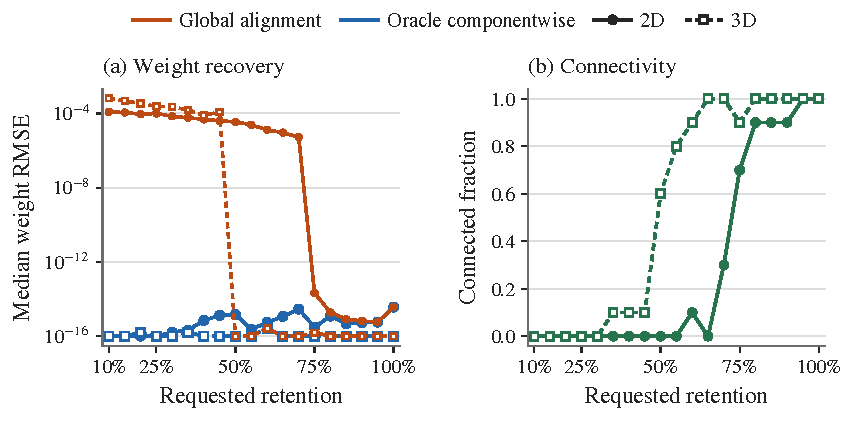
\includegraphics[width=\linewidth]{figures/figure_C_identifiability.pdf}
\caption{Missing observations without added noise (Experiment C), for $n=128$ in two and three dimensions. The horizontal coordinate is the requested retention fraction. Left: medians of per-run weight RMSE after one global alignment or separate componentwise alignments to the known generating weights. Values below $10^{-16}$ are floored for display on the logarithmic axis. Right: fraction of connected observation graphs. Each retention setting uses ten independently generated runs, so the curves are sampled profiles rather than nested deletion trajectories or universal connectivity thresholds.}
\label{fig:missing-observations}
\end{figure}

Observation error introduces a different difficulty even when the correct pair graph is known. Experiment B compares quadratic and Huber fitting under three noise conditions: Gaussian perturbations, Laplace perturbations, and sparse outliers on a Gaussian background. Accuracy is measured against the untouched generating separators, rather than against the corrupted fitting targets. The tested outlier cases show a modest benefit from Huber fitting. For example, in the two-dimensional setting with a nominal $5\%$ outlier fraction, the mean clean-reference separator RMSE is $0.00809$ for quadratic fitting and $0.00755$ for Huber fitting, in normalized-coordinate units. The benefit is not uniform across the Gaussian and Laplace settings; the noise levels, threshold and complete configuration are given in \ref{app:synthetic-noise}.

Hard restrictions raise a separate question: can they be satisfied simultaneously? As a short control, Experiment D correctly classifies all 30 generated three-observation cases as feasible or contradictory. It uses a dedicated experimental difference-constraint checker, distinct from the production fitting precheck; its construction is described in \ref{app:synthetic-controls}.

\subsection{Separator agreement and geometric realization}
\label{subsec:numerical-geometry}

A separator observation in a periodic system identifies both a site pair and a particular image. Experiment F asks what happens when that image information is wrong. In the noiseless control with the generating image shifts supplied, separator errors are near numerical precision and all requested faces are realized. Deliberately incorrect supplied shifts remain fixed during fitting: adjusting the weights does not revise the observation's image identity. A realized face at another image can therefore expose a mismatch that the fitted separator value alone does not resolve.

F also tests a separate image-selection procedure. It removes the image labels, chooses nearest images, and optionally revises them using uniquely realized shifts. In the three-dimensional tests, the revised choices all agree with their realized-image diagnostics, but only a fraction $0.924$ agree with the generating shifts. Geometric self-consistency is therefore insufficient to establish the correct periodic-image identity. This image-selection procedure is separate from the optional observation-set refinement, which retains the supplied shifts. Repeated stripped-label inputs and the exact scoring conventions are documented in \ref{app:synthetic-images}.

Experiment G instead keeps the generating diagram's neighbor pairs and alters their separator targets. Structured pair-dependent changes are added with amplitude $\eta$; the resulting targets need not be representable by one weight per site. The \emph{type-cycle} law encodes cyclic preferences among three site types, while the \emph{local-context} law uses contrasts in local neighbor spacing; their definitions are given in \ref{app:synthetic-mismatch}. We fit those targets and then compare the \emph{entire realized adjacency graph} with the generating graph. This tests whether closer agreement with local separator positions also preserves the reference neighbor relations. We summarize pair agreement by F1, the harmonic mean of precision (the fraction of realized pairs belonging to the reference) and recall (the fraction of reference pairs realized).

Figure~\ref{fig:model-mismatch} compares fitting accuracy and geometric recovery throughout the tested range of structured perturbations. The fit has lower error against the imposed separator targets than the ordinary Voronoi midpoint baseline at every tested amplitude. At $\eta=0$, when the targets come from a generating power diagram, the fitted diagrams have higher mean realized-graph F1; as the imposed targets are perturbed, this mean advantage reverses for both perturbation laws. The data at different amplitudes use independent configurations, so the trends are not trajectories of individual diagrams or universal mismatch thresholds.

\begin{figure}[!tbp]
\centering
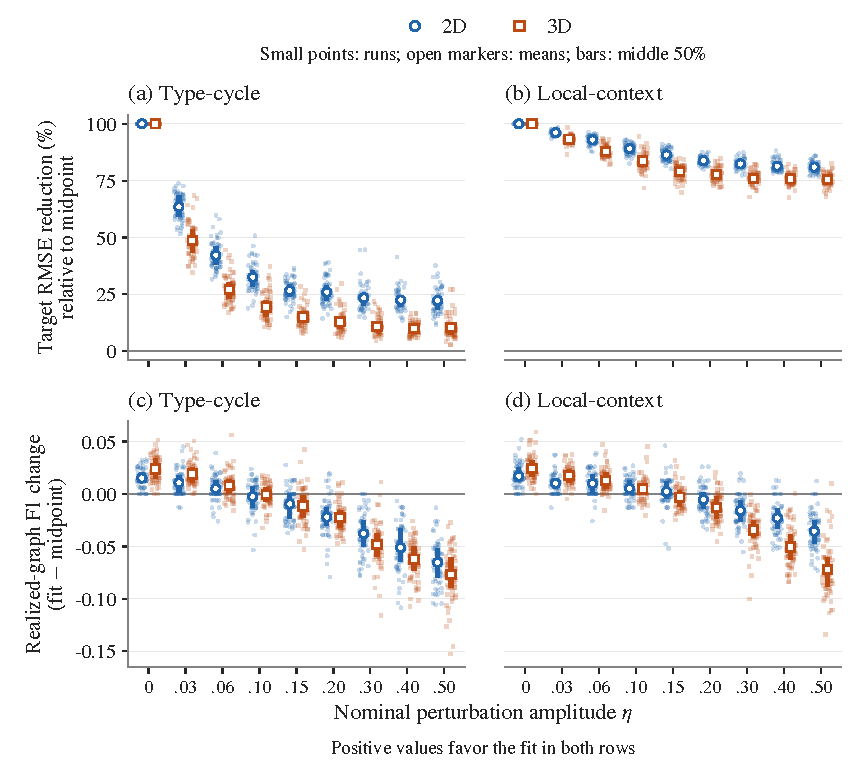
\includegraphics[width=\linewidth]{figures/figure_G_mismatch.pdf}
\caption{Target fitting and realized adjacency under structured mismatch (Experiment G). Columns show the two perturbation laws; circles and squares denote two and three dimensions. Each amplitude/dimension/law group contains 60 runs from two geometry families and three site counts. Top: percentage reduction in separator RMSE relative to midpoints, evaluated on the imposed fitting targets. Bottom: fitted minus midpoint F1 for the \emph{entire realized adjacency graph}, relative to the generating graph; positive values favor the fit in both rows. Faint points show runs, open markers their arithmetic means, and bars the middle 50\% of values (not confidence intervals). Nominal amplitudes are equally spaced for display, and instances at different amplitudes are independent. At $\eta=0.5$, target-coordinate clipping affects on average $38.25\%$ of type-cycle targets (\ref{app:synthetic-mismatch}).}
\label{fig:model-mismatch}
\end{figure}

At $\eta=0.2$, all 24 configuration groups have lower mean target RMSE after fitting, but also lower mean realized-graph F1. For example, among 60 two-dimensional type-cycle runs, the mean target RMSE is $0.109$ for the fit versus $0.147$ for midpoints, while mean realized-graph F1 is $0.961$ versus $0.983$. These are means of per-run scores. The midpoint baseline is itself an admissible equal-weight fit, and the same imposed targets enter both fitting and its error evaluation; lower in-sample target error therefore does not establish better recovery of the generating geometry. The perturbation laws and numerical protocol are detailed in \ref{app:synthetic-mismatch}.



\subsection{Optional refinement: benefits and failures}
\label{subsec:numerical-refinement}

The previous tests know which pairs supplied the generating diagram's separators. Experiments E and H add other pairs as candidates and ask whether the optional refinement can identify a more useful subset of observations. Every candidate set contains all generating neighbor pairs. In E, their targets receive small random errors, while the additional candidates receive approximate midpoint targets. H combines the enlarged candidate set with structured separator changes of the kind used in G.

We compare a one-pass fit using every candidate observation with the refined fit. For pair selection, the one-pass result selects candidates whose requested faces are realized; refinement selects the observations in its returned active set. Precision, recall and F1 compare these selections with the fixed set of generating neighbor pairs. Thus the scores concern selection among the candidates, rather than all adjacencies of the final diagram. Separator RMSE is evaluated on that same fixed reference-pair set, against clean generating separators in E and the imposed, potentially incompatible targets in H. All separator errors are in normalized-coordinate units.

\begin{table}[!htbp]
\centering
\footnotesize
\setlength{\tabcolsep}{4pt}
\caption{One-pass and refined fits in E and H. Values are arithmetic means of paired per-run scores. RMSE uses the fixed generating neighbor pairs, with clean targets in E and imposed targets in H; F1 scores the selected candidate observations. Counts classify the paired changes: lower RMSE or higher F1 is better. H includes the 72 positive-mismatch comparisons, excluding $\eta=0$.}
\label{tab:refinement-paired}
\begin{tabular}{@{}llrrrrr@{}}
\toprule
Study & Score & One pass & Refined & Better & Tied & Worse \\
\midrule
E (20) & RMSE & 0.00790 & 0.00385 & 19 & 0 & 1 \\
 & F1 & 0.99253 & 0.99479 & 4 & 15 & 1 \\
\cmidrule(lr){1-7}
H ($\eta>0$, 72) & RMSE & 0.13118 & 0.13422 & 70 & 0 & 2 \\
 & F1 & 0.96755 & 0.96701 & 19 & 32 & 21 \\
\bottomrule
\end{tabular}
\end{table}

In E, refinement approximately halves the mean error against clean separators, while the already high mean pair-selection F1 changes little (Table~\ref{tab:refinement-paired}). All 20 refinements reach the implemented self-consistency condition. The main benefit in these instances is therefore more accurate separator positions; it is not a substantial improvement in pair selection.

\Needspace{10\baselineskip}
H shows why frequent improvements and a favorable mean need not coincide. Error decreases in 70 of the 72 positive-mismatch comparisons, yet its mean increases because of a severe adverse case. One run worsens from $0.1266$ to $0.6929$ with unchanged pair-selection F1 and stops after a previously seen active set recurs. Across all 96 H refinements, including zero mismatch, 85 stop on the implemented self-consistency test and 11 after an active set recurs. The recorded final inner fits have optimal status, but the recurrence of an active set does not establish convergence of the outer updates. The error, selected pairs and stopping outcome must therefore be assessed separately.

% SOURCE A--D: results/{exact_recovery,noise_robustness,missing_data_manuscript,infeasible}/.
% SOURCE F/G: results/{periodic,model_mismatch}/ and their experimental generators.
% SOURCE E/H: results/{active_set,supergraph_mismatch}/runs.csv; paired
% by seed and configuration in scripts/check_manuscript_tables.py. H uses
% eta>0; stopping counts use all 96 refinements. The absolute tie tolerance
% is 1e-12 on unrounded score changes. See manuscript/README.md evidence map.
% Figure C: scripts/plot_editorial_figures.py reads the frozen runs.csv;
% no simulation, fitting or solver result is recomputed.

\section{A molecular application}
\label{sec:molecular-application}
\label{subsec:numerical-molecular}

Atomic systems are a natural application of space partitions: the nuclei supply fixed sites, and cells assign a region of space to each atom. Voronoi-based constructions have long been used to study atomic volumes and molecular packing \cite{Richards1974}. Ordinary Voronoi cells place each pairwise dividing plane halfway between the nuclei, independently of their species or electronic environment. Radius-dependent radical, or power, diagrams allow unequal atomic sizes \cite{GellatlyFinney1982}; more recent work also optimizes their radii using electron-density integrals and fluctuations of atomic and molecular charges \cite{BrehmThomas2021}. The question for an inverse construction is therefore which physical observations should determine the weights.

The Quantum Theory of Atoms in Molecules (QTAIM) supplies a physically motivated reference partition. It divides the electron density into basins whose gradient-ascent paths lead to the same attractor, usually associated with a nucleus \cite{Bader1980,Bader1990}. Along their boundaries the density gradient has zero normal component. This zero-flux condition has a quantum-mechanical justification in Bader's formulation of atoms as open subsystems \cite{Bader1994}. Basin integrals give atomic electron populations and charges, while the density's gradient-path network describes relations between atomic regions \cite{Bader1990}. Thus this partition provides both integral quantities and local geometric information to approximate.

Here we ask how much of that local information a power diagram can represent while keeping the nuclei fixed. Related inverse problems use cell volumes and centroids as data \cite{BournePearceRoper2025}. Our aim is instead to locate selected interatomic separators and examine which pairs acquire shared faces. Approximating the full curved boundaries would require more extensive boundary information, such as surface samples, and a specified measure of discrepancy. We use a simpler available observation: a \emph{bond critical point} (BCP), a density saddle on an interatomic boundary from which two gradient-ascent branches lead toward the neighboring atomic attractors \cite{Bader1980}.

For the connector-normal plane family fixed by the nuclear positions, a BCP specifies one target offset. Its orthogonal projection onto the connector defines a target plane that also passes through the original point. Fitting these offsets reconciles local boundary landmarks into one set of atomic weights; it need not preserve every target exactly. Nor does a plane through a landmark necessarily give the best approximation to a whole curved interface. Figure~\ref{fig:bcp-projection} illustrates the projection and the curved boundary; \ref{app:molecular-background} gives the physical background and experimental protocols.

The benchmark contains 100 molecules and 3,975 BCP-supported reference pairs (Experiment J1). Of these, 3,703 are bonded and 272 nonbonded, where \emph{bonded} means adjacency in the explicit-hydrogen RDKit molecular graph \cite{RDKit2026}. Both groups contain BCPs; their names refer to this separate connectivity convention. We report them separately because pooled scores are dominated by the bonded pairs. The experiments first examine separator accuracy on the known reference pairs, then replace that input with distance-selected candidates, and finally assess the information supplied by local geometric diagnostics. Their measured outputs are separator locations and pair labels, rather than complete QTAIM basin shapes or volumes.

\subsection{Separator fitting on known atom pairs}
\label{subsec:molecular-known-pairs}

Experiment J2 assumes that the QTAIM-supported pair graph is known. We compare ordinary midpoints with a local \emph{proatomic} prediction, which locates a minimum of the sum of two radial atomic density profiles along the nuclear connector for unlike atoms and uses the midpoint for homonuclear pairs. A one-pass weight fit reconciles these proatomic observations using a single weight per atom. A separate \emph{QTAIM-target reference fit} instead fits the projected BCP coordinates directly, testing how those landmarks can be represented on the same known pair graph.

Table~\ref{tab:molecular-fits} evaluates all four models on the original reference pairs, without filtering by face realization. Errors are measured in \AA{} and pooled over the individual pairs in each stated subset. The QTAIM-target fit itself minimizes the unweighted squared error in \emph{normalized coordinates}, over the full reference graph of each molecule; the displayed length errors and subset errors are consequently different evaluation quantities. Further predictor and aggregation details are in \ref{app:molecular-protocols}.

\begin{table}[htbp]
\centering
\footnotesize
\setlength{\tabcolsep}{4pt}
\caption{Separator RMSE in \AA{} on fixed QTAIM-supported pair subsets (J2). The two fitted models use the known reference-pair graph. The direct QTAIM-target fit minimizes unweighted squared error in normalized coordinates over each molecule's full reference graph. All displayed length errors are pooled over pairs.}
\label{tab:molecular-fits}
\begin{tabular}{@{}lrrrr@{}}
\toprule
Subset & Midpoint & Proatomic & Proatomic fit & QTAIM-target fit \\
\midrule
All & 0.1332 & 0.0452 & 0.0473 & 0.0169 \\
Bonded & 0.1317 & 0.0457 & 0.0461 & 0.0062 \\
Nonbonded & 0.1528 & 0.0372 & 0.0619 & 0.0605 \\
\bottomrule
\end{tabular}
\end{table}

The local proatomic predictor has substantially smaller RMSE than midpoint prediction. Enforcing a common weight representation nevertheless increases the overall error slightly and the nonbonded error more markedly, from $0.0372$ to $0.0619$~\AA{}. Both fitted models realize every requested reference pair, so the deterioration is not caused by losing difficult pairs from the evaluation. The direct QTAIM-target fit also leaves a larger nonbonded than bonded error. These results distinguish the accuracy of a local predictor from the accuracy retained when its outputs are reconciled into one power diagram. The nonbonded QTAIM-target value is consequently not a lower bound on attainable length error for that subset.

\subsection{Fitting from candidate pairs}
\label{subsec:molecular-candidates}

Experiment J3 removes the assumption that the reference pairs are known during fitting. Candidate pairs are selected by distance, with cutoffs of $4$, $4.5$ and $5$~\AA{}, and receive proatomic separator predictions. Each cutoff contains all 3,975 reference pairs. Increasing the cutoff therefore adds other observations without increasing reference coverage. The reference-pair RMSE of the resulting one-pass fit rises from $0.0746$ to $0.0786$~\AA{} between the smallest and largest cutoff. All reference pairs are realized and included in these errors. The complete cutoff comparison is given in Table~\ref{tab:molecular-candidates}.

We then examine which realized pairs agree with the QTAIM reference. This evaluation uses the entire realized adjacency graph, including pairs outside the input candidate set. Connector visibility is applied afterwards as a geometric filter, using the tolerance-inclusive membership test on clipped faces specified in \ref{app:molecular-candidates}. At the $5$~\AA{} cutoff, it retains 5,703 pairs, including 3,973 of the 3,975 reference pairs: visible precision is $0.697$ and recall is $0.9995$. The aggregate result conceals a substantial difference between pair classes. Bonded recovery is nearly exact (F1 approximately $0.9997$); among the retained nonbonded pairs, only $13.5\%$ belong to the reference set. Thus almost all reference pairs are retained, but many additional nonbonded pairs remain. These additional pairs are absent from the adopted BCP-supported reference set; that label alone does not determine whether a contact has chemical significance.

J3 uses one-pass fitting followed by geometric filtering. It does not update the fitted observation set through the optional refinement of Section~\ref{subsec:workflow-active-mask}. The next experiment asks whether clearance provides information beyond the binary visibility decision.

\subsection{Geometric diagnostics for nonbonded contacts}
\label{subsec:molecular-diagnostics}

A visible connector point may lie near the boundary of its clipped face or well inside it. Experiment J4b tests whether the clipped connector-centered clearance $c_{ij}^{\Omega}$ from Eq.~\eqref{eq:clipped-clearance} helps distinguish QTAIM-supported from additional pairs among the \emph{already visible nonbonded faces}. Clearance and face area are measured in the reference box, formed by padding the atomic-coordinate bounding box by $5$~\AA{}. We rank faces by larger clearance, shorter pair distance or larger face area. Average precision (AP) summarizes how well each ranking places reference pairs ahead of additional pairs; its definition and eligible populations are specified in \ref{app:molecular-diagnostics}.

Table~\ref{tab:molecular-clearance-ranking} pools eligible faces across molecules, separately for an ordinary Voronoi diagram and the J3 power fit at $5$~\AA{}. Within each population, clearance has higher AP than distance or area. For the fitted-power population, median clearance is $0.678$~\AA{} on reference pairs and $0.228$~\AA{} on additional pairs. The two models have different eligible populations, so the comparisons among ranking variables are made within each row of the table.

\begin{table}[htbp]
\centering
\footnotesize
\setlength{\tabcolsep}{4.5pt}
\caption{Pooled average precision for ranking QTAIM-supported pairs above additional visible nonbonded pairs (J4b). Larger clipped clearance and face area in the reference box, and shorter pair distance, give higher ranks. Each model has its own eligible population; the AP values compare ranking variables within that population and do not provide a common-population comparison between the two models.}
\label{tab:molecular-clearance-ranking}
\begin{tabular}{@{}lrrrrr@{}}
\toprule
Model & Visible pairs & QTAIM+ & Clearance AP & Short-dist. AP & Area AP \\
\midrule
Voronoi & 2,269 & 258 & 0.707 & 0.641 & 0.150 \\
Power fit & 1,998 & 270 & 0.830 & 0.636 & 0.161 \\
\bottomrule
\end{tabular}
\end{table}

Checks on the recorded realized faces also confirm agreement between the analytic visibility and clipped-clearance calculations and the tessellation-based diagnostics (J4a; \ref{app:molecular-diagnostics}). The ranking result is a pooled comparison, rather than a statement about every individual molecule. It shows that clearance supplies additional discriminatory information within these visible-face populations, where binary visibility alone retains many nonbonded pairs outside the reference.

% SOURCE J1--J4: frozen results/qtaim_main/{J1_dataset_audit,
% J2_true_support_ladder,J3_candidate_recovery_refresh,
% J4_local_diagnostic_validation,J4_mask_transfer_refresh}/.
% J2/J3 length errors are pooled over edge records. The direct BCP fit
% minimizes full-graph fraction-space loss separately for each molecule.
% J3 evaluates the entire realized graph and performs no outer refinement.
% J4b AP populations differ. J4c/J4d protocol limits are in Appendix E.

\section{Discussion}
\label{sec:discussion}

Applying the fixed-site separator model begins with deciding what the observations represent. A measured interface point and a numerical prediction can supply the same kind of offset while carrying different uncertainties and biases. The sites fix the plane's orientation, so fitting its offset alone does not establish agreement with the orientation or curvature of a physical interface. Measurement units and fitting weights should therefore reflect the intended discrepancy. Pair assignments require the same care: in periodic problems, a selected image is part of an observation's identity. The image tests in Section~\ref{subsec:numerical-geometry} show that agreement with the fitted diagram's realization diagnostics does not establish that the intended images were chosen.

Incomplete observations leave ambiguities that improved numerical accuracy cannot resolve. The deletion experiment in Figure~\ref{fig:missing-observations} preserves accurate relative weights within each connected component while losing their relation to other components. Choosing the missing offsets selects a diagram; additional observations or suitable constraints are needed to restrict those choices. Even with a connected observation graph, sensitivity to noise depends on its structure and fitting weights. The deterministic estimates in \ref{app:stability-details} describe that response for a fixed fitting problem, but do not supply a statistical uncertainty model for a new source of observations.

Fitting error also answers a different question from agreement with an independent reference. In Figure~\ref{fig:model-mismatch}, closer agreement with altered separator targets accompanies poorer recovery of the generating adjacency graph. In the molecular comparison, reconciling local proatomic predictions increases the pooled nonbonded separator RMSE from $0.0372$ to $0.0619$~\AA{}, although every requested reference pair remains realized (Table~\ref{tab:molecular-fits}). The fitting objective and reported subset length errors differ, so this does not isolate an unavoidable loss due to compatibility alone. These examples make independent evaluation essential: neither a smaller fitting residual nor successful face realization establishes fidelity to the intended reference geometry.

Local support needs a similarly specific interpretation. Connector membership checks whether a face contains the separator's intersection with the line through its sites; it does not assess the entire face's agreement with a physical boundary. In the molecular experiments, the test uses clipped faces and a tolerance that admits boundary cases beyond strict positive-margin visibility. It retains almost all reference pairs but also many additional nonbonded pairs. Among the visible nonbonded faces, clearance helps distinguish reference pairs within each model's evaluated population (Table~\ref{tab:molecular-clearance-ranking}), yet supplies neither a universal selection threshold nor a chemical interpretation of every additional pair. Domain clipping and periodic competitors must likewise enter the geometric checks in other applications.

Optional refinement introduces a further empirical choice. Its face-driven changes to the fitted observation set improve separator accuracy in the clean-reference comparison of Section~\ref{subsec:numerical-refinement}. With structured mismatch, error against the imposed targets decreases in most paired comparisons, yet its mean increases because of a severe adverse case. Refinement therefore requires evaluation of the returned errors, selected observations and final geometry alongside the stopping outcome. Optimality of a final inner fit does not establish convergence of the outer updates, and recurrence of an observation set is only the implemented stopping diagnostic. The one-pass construction provides the baseline for assessing this optional step.

Other sources of local separator information, such as sampled interfaces or landmarks of physical fields, can be treated through the same observation model when pair assignments and fixed plane orientations are meaningful. Each application still needs its own criterion for assessing the resulting partition against the geometry or physical quantities it is intended to represent.

\section{Conclusions}
\label{sec:conclusions}

This work provides a reproducible method for fitting power diagrams to selected numerical separator observations at fixed sites. The affine relation between separator positions and weight differences reduces exact compatibility and identifiability to graph conditions, and unconstrained quadratic fitting to a weighted graph-Laplacian problem. Compatible observations determine relative weights within each connected component; a connected observation graph determines all weights up to a common shift that leaves the diagram unchanged. Synthetic tests with exact compatible data recover these observable differences to numerical precision and show how missing observations limit reconstruction.

Geometric assessment asks whether the cells share a face and whether it contains the fitted plane's intersection with the line through the sites. When this point lies inside the face, centered clearance measures its in-plane distance to the boundary. For finite nonperiodic configurations, a strict power-distance advantage of the pair over all competing sites at this point certifies a face nearby, and the perturbation bounds give sufficient conditions for retaining that local advantage. Clipping and periodicity require the corresponding domain and image checks.

The experiments show that agreement with supplied separators and with an independent reference can diverge. In synthetic tests, better target fitting can accompany poorer recovery of reference adjacencies. In the 100-molecule application, fits using the known reference pairs realize all their requested faces, although reconciling local predictions from atomic density profiles does not necessarily improve separator accuracy against electron-density landmarks. With distance-selected candidates, connector-visibility filtering retains 3,973 of the 3,975 reference pairs, together with additional nonbonded pairs. Centered clearance adds further information: among visible nonbonded faces, it ranks density-supported reference pairs more effectively than distance or face area within each model's evaluated population. These findings concern local separator positions and pair relations; complete electron-density basins have not been reconstructed or validated.

Optional face-driven refinement improves accuracy in some tests and degrades it in others, and its stopping diagnostics do not establish general convergence. The main outcome is a method for turning incomplete local separator information into a global power diagram whose identifiable weight information, realized faces and local geometric support can each be examined explicitly.



\section*{Code, data, and manuscript availability}
The scripts, experimental configurations, and numerical results underlying this
work are preserved in the \texttt{powerfit} version~1.0.0 archive
\cite{PowerfitArchive2026}. The all-versions \texttt{powerfit} record
\cite{PowerfitProject2026} provides a persistent link to the latest published
project release, including manuscript revisions and accompanying
reproducibility materials. The fitting and tessellation calculations reported
here used \texttt{pyvoro2} version~0.6.3 \cite{Pyvoro2_063}.

\section*{Acknowledgments}
The author thanks Chris H. Rycroft for helpful discussions and constructive
feedback on an earlier version of this manuscript, which motivated a
substantial reorganization of its exposition. The author is deeply grateful
to his mother for her unconditional support during a difficult period.

\section*{Declaration of generative AI and AI-assisted technologies}
During the preparation of this work, the author used GPT (OpenAI) to assist with
manuscript planning, drafting and editing, mathematical and editorial review,
source-code inspection and development, and the checking and interpretation
of archived computational results. The author remains responsible for the
research design, scientific claims, numerical evidence and conclusions.

\bibliographystyle{elsarticle-num}
\bibliography{refs}

\appendix
\counterwithin*{figure}{section}
\counterwithin*{table}{section}
\section{Supplementary graph and optimization arguments}
\label{app:graph-optimization}

Here we prove that the constrained quadratic fit in Eq.~\eqref{eq:hard-constrained-fit} attains its minimum and describe all its minimizers.

% Editorial note: This appendix is provisional and subject to the Section 3
% independent Pro audit. Expand it only where the main text requires more
% formal support. See notes/appendix_backlog_2026-10-18.md.
% APPENDIX-TODO [app:graph-multigraph]: Optional incidence/cycle-space details.
% APPENDIX-TODO [app:graph-gauges]: Component gauges versus geometric gauge.
% APPENDIX-TODO [app:graph-statistics]: Covariance/precision interpretation.
% APPENDIX-TODO [app:graph-convexity]: General robust-loss hypotheses.
% APPENDIX-TODO [app:graph-differences]: Optional numerical feasibility scope.

\subsection{Attainment of the constrained quadratic fit}
\label{app:constrained-attainment}

\begin{proof}
Assume $R$ is positive diagonal and the hard-feasible set $\mathcal H$
in Eq.~\eqref{eq:hard-feasible-set} is nonempty. Put
$T=R^{1/2}B^T$ and $a=R^{1/2}z$. Then the objective is
$\frac12\|Tw-a\|_2^2$. Since $\mathcal H$ is a polyhedron,
its linear image $T(\mathcal H)$ is also a polyhedron
\cite[Theorem~19.3]{Rockafellar1970} and hence
a nonempty closed convex subset of $\mathbb R^m$.
The Euclidean projection of $a$ onto $T(\mathcal H)$ exists.
Every point of $T(\mathcal H)$ has a feasible preimage by its
definition, so choosing one preimage of this projection gives
a minimizer of Eq.~\eqref{eq:hard-constrained-fit}.
To characterize all minimizers, let $w^\star\in\mathcal H$ be one
of them. The Euclidean projection onto $T(\mathcal H)$ is unique,
so another feasible weight vector $w$ minimizes the same objective
if and only if $Tw=Tw^\star$. Since $R$ is positive diagonal,
$\ker T=\ker B^T$. Consequently,
\begin{equation}
\operatorname*{argmin}_{w\in\mathcal H}\mathcal E(w)
=\mathcal H\cap\bigl(w^\star+\ker B^T\bigr).
\label{eq:constrained-minimizer-set}
\end{equation}
Thus, hard restrictions can limit the componentwise offsets
between fitting minimizers, while a common additive shift of all
site weights always remains possible.
\end{proof}

\section{Geometric support, degeneracies, and domains}
\label{app:geometric-details}

We first examine how ties affect connector visibility and face dimension, then distinguish clearance at a connector point inside the face from distance to the face when that point lies outside it. The last two subsections explain how clipping and selected periodic images affect these checks.


\subsection{Weak visibility, persistent ties, and face dimension}
\label{app:geometry-degeneracy}

Consider a finite set of distinct sites in $\mathbb R^d$ with finite real weights. Fix $i\ne j$, and let $q=q_{ij}$ and $H=H_{ij}$ be the pairwise connector point and bisector defined in Section~4. Every point $x\in H$ can be written $x=q+u$ with $u\cdot\delta_{ij}=0$. As in Eq.~\eqref{eq:power-gap-displacement}, the competing-site inequalities restricted to $H$ are
\begin{equation}
2e_{ijk}\cdot u\le g_{ijk},
\qquad k\notin\{i,j\}.
\label{eq:appendix-face-halfspaces}
\end{equation}
Thus the common cell intersection is a (possibly empty or unbounded) closed convex polyhedron within $H$.

Weak connector visibility, $g_{ijk}\ge0$ for all $k$, is exactly the condition $q\in F_{ij}$; it need not imply that $q$ lies in the interior within the \emph{full} $(d-1)$-dimensional hyperplane $H$. Conversely, strict positivity of every competitor gap suffices for such interior membership, but is not necessary in the presence of persistent ties.

In particular, when $e_{ijk}=0$, inequality~\eqref{eq:appendix-face-halfspaces} is constant throughout $H$. If $g_{ijk}<0$, it excludes the entire bisector; if $g_{ijk}>0$, it imposes no restriction on the face; if $g_{ijk}=0$, it is an equality throughout $H$ and does not reduce the extent of $F_{ij}$ \emph{within} the bisector. In contrast, when $g_{ijk}=0$ and $e_{ijk}\ne0$, the corresponding halfspace boundary within $H$ passes through $q$. No ball of positive radius centered at $q$ within $H$ can then be contained in $F_{ij}$.

For an explicit persistent tie, take $p_i=(0,0)$, $p_j=(2,0)$, $p_k=(1,0)$ and $(w_i,w_j,w_k)=(0,0,-1)$. At every point of $H_{ij}=\{(1,y):y\in\mathbb R\}$, all three power distances agree. Consequently $F_{ij}=H_{ij}$ and $q_{ij}\in\operatorname{int}_{H_{ij}}F_{ij}$, yet $g_{ijk}=0$ identically. Here $C_i=\{(x,y):x\le1\}$ and $C_j=\{(x,y):x\ge1\}$ are full-dimensional cells sharing a facet, but the degenerate cell $C_k=H_{ij}$ also minimizes power there. Thus interior membership does not exclude a third minimizing site or imply strict visibility. If instead the selected pair is $i,k$, then $F_{ik}=H_{ik}=H_{ij}$ while $C_k$ has empty ambient interior; full-dimensionality of the intersection within its bisector does not by itself certify that both selected cells are full-dimensional.

We always use $\operatorname{int}_{H_{ij}}$, the interior relative to the \emph{entire pairwise bisector}, not the ordinary relative interior within $\operatorname{aff}(F_{ij})$. The latter is nonempty for every nonempty convex face, including a singleton, and would fail to distinguish full-dimensional interfaces.

\subsection{Centered clearance and exterior distance to a face}
\label{app:geometry-exterior}

The gap inequalities~\eqref{eq:appendix-face-halfspaces} also describe the distance to a realized face when the connector point itself is not feasible. Define
\begin{equation}
V_{ij}=\left\{u\in\delta_{ij}^{\perp}:
2e_{ijk}\cdot u\le g_{ijk}
\text{ for all }k\notin\{i,j\}\right\}.
\label{eq:face-displacement-feasible-set}
\end{equation}
Then
\begin{equation}
F_{ij}=q_{ij}+V_{ij}.
\label{eq:face-displacement}
\end{equation}
The set $V_{ij}$ is a closed convex polyhedron, possibly empty.

\paragraph{Interior clearance}
If $q_{ij}\in F_{ij}$, the largest radius of a closed Euclidean ball \emph{within} $H_{ij}$ centered at $q_{ij}$ and contained in $F_{ij}$ satisfies
\begin{equation}
c_{ij}=
\min_{\substack{k\notin\{i,j\}\\\|e_{ijk}\|>0}}
\frac{g_{ijk}}{2\|e_{ijk}\|},
\label{eq:weak-centered-clearance}
\end{equation}
with the minimum of an empty set interpreted as $+\infty$. Indeed, the minimum of each affine gap over the centered ball of radius $r$ is $g_{ijk}-2r\|e_{ijk}\|$; all these values must be nonnegative. The same argument works when $\sigma_{ij}=0$, not only when it is positive. A zero gap with nonzero $e_{ijk}$ forces $c_{ij}=0$; a zero gap with $e_{ijk}=0$ imposes no in-bisector restriction. When no constraint has a nonzero projected normal and $q_{ij}\in F_{ij}$, the whole bisector is contained in the face and $c_{ij}=+\infty$. Redundant halfspaces do not affect this derivation.

\paragraph{Exterior distance}
If $q_{ij}\notin F_{ij}$ but $F_{ij}\ne\varnothing$, define its \emph{exterior face distance} as the inherited Euclidean distance within the bisector,
\begin{equation}
d_{ij}^{\mathrm{out}}
=\operatorname{dist}_{H_{ij}}(q_{ij},F_{ij}).
\label{eq:exterior-face-distance}
\end{equation}
Using~\eqref{eq:face-displacement}, this distance is computed by the convex quadratic program
\begin{equation}
\boxed{
\begin{aligned}
(d_{ij}^{\mathrm{out}})^2
&=\min_{u\in\delta_{ij}^{\perp}}\|u\|^2,\\
\text{subject to}\quad
&2e_{ijk}\cdot u\le g_{ijk}
\qquad\text{for all }k\notin\{i,j\}.
\end{aligned}}
\label{eq:exterior-distance-qp}
\end{equation}
For a nonempty face the minimum is attained at a unique point: this is Euclidean projection onto a nonempty closed convex set. If the inequalities are infeasible, $F_{ij}=\varnothing$ and the standard distance-to-set convention gives $d_{ij}^{\mathrm{out}}=+\infty$; there is then no nearest point. The quantity measures distance to the \emph{specified pair's face}, not to the closest face of any site pair in the full diagram.

\paragraph{Why negative clearance ratios are not exterior distances}
Consider the formal algebraic extension
\begin{equation}
\widetilde c_{ij}=
\min_{\|e_{ijk}\|>0}\frac{g_{ijk}}{2\|e_{ijk}\|}.
\label{eq:formal-negative-clearance}
\end{equation}
For a violated inequality with nonzero projected normal, the positive quantity $-g_{ijk}/(2\|e_{ijk}\|)$ is the distance from $q_{ij}$ to the feasible \emph{halfspace for that single inequality}. The full face is the intersection of all halfspaces, so its distance from $q_{ij}$ can exceed each individual halfspace distance, and the intersection itself may be empty. Constant violated inequalities ($e_{ijk}=0,\ g_{ijk}<0$) are another obstruction: they make the whole face empty without appearing in~\eqref{eq:formal-negative-clearance}.

An explicit example with a nonempty face occurs in $\mathbb R^3$. Take
\begin{equation}
\begin{aligned}
p_1&=(0,0,0), & p_2&=(2,0,0),\\
p_3&=(1,-1,0), & p_4&=(1,0,-1),
\end{aligned}
\qquad
(w_1,w_2,w_3,w_4)=(0,0,2,2).
\label{eq:exterior-counterexample}
\end{equation}
Here $H_{12}=\{(1,y,z)\}$, $q_{12}=(1,0,0)$, and the two competitor inequalities require $y\ge1$ and $z\ge1$. The face is the nonempty quadrant $\{(1,y,z):y\ge1,\ z\ge1\}$, so
\begin{equation}
\widetilde c_{12}=-1,
\qquad d_{12}^{\mathrm{out}}=\sqrt2.
\label{eq:exterior-example-values}
\end{equation}
In the four-site configuration of Eq.~\eqref{eq:four-sites} with $(w_3,w_4)=(1,1)$, the face is instead empty despite a finite negative formal ratio. Hence a negative continuation of the centered-clearance formula cannot be identified with a signed distance to the true face. The centered interior radius and the distance to a realized face are therefore distinct geometric quantities.

\subsection{Clipping to a convex box}
\label{app:geometry-clipping}

For a convex box or, more generally, a fixed convex polytope
\begin{equation}
\Omega=\{x\in\mathbb R^d:a_\ell\cdot x\le b_\ell
\text{ for all }\ell\},
\label{eq:domain-halfspaces}
\end{equation}
the clipped intersection is $F_{ij}^{\Omega}=F_{ij}\cap\Omega$. Each domain inequality restricted to $x=q_{ij}+u\in H_{ij}$ takes the form
\begin{equation}
a_\ell\cdot u\le b_\ell-a_\ell\cdot q_{ij}.
\end{equation}
Let $P_{ij}$ be orthogonal projection onto $\delta_{ij}^{\perp}$. When $q_{ij}\in\Omega$, the largest radius of a centered in-bisector ball contained in $\Omega$ is
\begin{equation}
b_{ij}^{\Omega}=
\min_{\ell:\|P_{ij}a_\ell\|>0}
\frac{b_\ell-a_\ell\cdot q_{ij}}{\|P_{ij}a_\ell\|},
\label{eq:box-inplane-radius}
\end{equation}
with empty minimum $+\infty$; a constraint with zero projected normal has no effect on motion within $H_{ij}$ when already satisfied at $q_{ij}$.

If $q_{ij}\in F_{ij}\cap\Omega$, the centered radius of the clipped intersection is exactly $\min\{c_{ij},b_{ij}^{\Omega}\}$ by the two families of halfspace inequalities. The strict-visibility and interior-domain hypotheses in Section~4.4 guarantee that this value is positive; at the boundary, ties and domain-wall coincidences require explicit attention.

When a domain wall coincides with $H_{ij}$, a clipped intersection may have nonempty $(d-1)$-dimensional interior within $H_{ij}$ without forming an interface between two full-dimensional cells \emph{inside} $\Omega$. An interior-domain strict witness is a sufficient way to exclude this boundary-only behavior, but not a necessary condition for every useful clipped geometric intersection. No analogous finite halfspace formula is claimed here for arbitrary nonconvex clipping domains.

\subsection{Selected periodic images and competitor scope}
\label{app:geometry-periodic}

For a fixed lattice with translations $\Lambda t$, a geometric site instance has position $p_{k,t}=p_k+\Lambda t$ and retains base weight $w_k$. A periodic pair observation specifies two \emph{selected instances}, such as $(i,0)$ and $(j,s)$. The bisector and its connector point are computed for those instances; their competitors are \emph{all other instances}. In particular, other copies of base sites $i$ or $j$ must not be discarded merely because their base indices match one of the endpoints. Distinct base sites may be equivalent modulo the lattice: a coincident \emph{unselected} image produces a constant competitor power-gap inequality, which is redundant, excludes the selected cell, or creates a persistent tie depending on its sign. The observed selected endpoints must still be distinct as required in Section~2.

The same affine pointwise power inequalities and in-bisector projection arguments apply to each selected instance and competitor. However, an infinite collection of image inequalities is not automatically a finite polyhedron, and an arbitrary neighbor-image stencil does not establish a complete exact realization test or a uniform finite stability constant. An exact finite reduction requires a justified region of interest and relevant-image bound.

Let $V=\operatorname{span}\Lambda$ and let $P_V$ denote orthogonal projection onto $V$. Competition with a selected site's own images confines $P_V(x-p_i)$, for every $x$ in that image's power cell, to the compact lattice Voronoi region in $V$. For images of any competing base site, the $V^\perp$ component of squared distance is independent of the shift, and all images share the same weight. Thus, for each competing base site, its nearest image depends only on $P_Vx$, and finitely many shifts suffice over the compact projected region even when the nonperiodic directions are unbounded. This supplies a route to a finite relevant-image reduction for selected cells and their faces under fixed partial periodicity.

It does not justify an arbitrary fixed image stencil or a uniform competitor set for connector points that move without restriction as weights change. Changing lattice geometry also requires separate control. Section~4 therefore does not extend its finite-competitor stability estimate to an unrestricted periodic theorem.

\section{Perturbation estimates for fitted weights and geometric diagnostics}
\label{app:stability-details}

We begin with the response of signed competitor gaps to weight perturbations, then propagate observation errors through a fixed least-squares fit. The remaining subsections account for discrepancies between the reference fit and independently specified weights, and state the competitor assumptions needed in periodic domains.

% Revised after independent Pro Run 1; pending correction verification.
% Fixed graph, fixed positive precisions, finite competitor set, and
% identifiable component gauges are essential hypotheses.
% No general guarantee for the changing active-mask iteration is asserted.

\subsection{Fixed-site signed-gap stability}
\label{app:stability-slack}

For a fixed finite competitor set, Eq.~\eqref{eq:gap-weight-perturbation} gives an exact affine change in each gap with coefficient sum zero, so a common global shift of the weights leaves all gaps invariant. The minimum-gap bound~\eqref{eq:gap-lipschitz-bound} follows from the elementary inequality $|\min_k a_k-\min_k b_k|\le\max_k|a_k-b_k|$.

Invariance under a common weight shift sharpens the bound to
\begin{equation}
|\sigma_{ij}(w+\Delta w)-\sigma_{ij}(w)|
\le K_{ij}\inf_{\gamma\in\mathbb R}
\|\Delta w-\gamma\mathbf1\|_\infty.
\label{eq:gap-gauge-invariant-lipschitz}
\end{equation}
Only the \emph{global} constant may be removed here: shifting disconnected components of the fitting graph separately need not preserve the full power diagram or its gaps. If the competitor set is empty, $\sigma_{ij}=+\infty$ by convention and the ordinary finite Lipschitz inequality is not applied.

For a finite competitor set, any nonzero reference gap with perturbation bound smaller than its absolute value retains its sign. This is a certificate for the chosen \emph{connector-visibility} diagnostic, not a statement that all faces or all combinatorial adjacencies of the power diagram persist.

\subsection{Sensitivity of a fixed weighted least-squares fit}
\label{app:stability-estimator}

Let $B\in\mathbb R^{n\times m}$ be the incidence matrix of a \emph{fixed} observation graph, let $R=\operatorname{diag}(\rho_r)$ have strictly positive entries, and put $L=BRB^T$. Suppose $\operatorname{rank}(B)=n-c>0$, where $c$ is the number of observation-graph connected components. Let $Q\in\mathbb R^{n\times(n-c)}$ have orthonormal columns spanning $(\ker B^T)^\perp$. Choosing this subspace is equivalent to a zero-mean convention within each observation component.

On this identifiable subspace, the reduced matrix $Q^TLQ$ is positive definite. For a target vector $z$, the unique least-squares solution with zero mean in each observation component is
\begin{equation}
w(z)=Gz,\qquad
G=Q(Q^TLQ)^{-1}Q^TBR.
\label{eq:fixed-fit-response-operator}
\end{equation}
For a reference target $z^\star$ (possibly incompatible) and perturbed target $\widehat z=z^\star+\eta$, define $w^\star=Gz^\star$ and $\widehat w=G\widehat z$. The exact response identity is
\begin{equation}
\widehat w-w^\star=G\eta.
\label{eq:appendix-reference-fit-response}
\end{equation}

This statement does \emph{not} identify $w^\star$ with an arbitrary independently chosen vector of true physical weights. It relates two minimizers of the \emph{same} fixed quadratic fitting problem evaluated at different target vectors, with the same component-offset convention. Other fixed linear gauges admit analogous expressions. A constant nonzero offset convention adds an affine constant to $w(z)$ but does not alter the response to $\eta$.

Write $\|v\|_L=(v^TLv)^{1/2}$ for the Laplacian seminorm. The fitted difference perturbation is a weighted orthogonal projection of $\eta$ onto the column space of $B^T$, giving
\begin{equation}
\|\widehat w-w^\star\|_L
\le\|R^{1/2}\eta\|_2.
\label{eq:energy-error-bound}
\end{equation}
To see this, put $A=R^{1/2}B^TQ$. The vector
$R^{1/2}B^T(\widehat w-w^\star)$ is the orthogonal projection of
$R^{1/2}\eta$ onto $\operatorname{range}(A)$, and therefore cannot have
larger Euclidean norm.

If the observations are perturbed by $\Delta y_r$ in their original measurement units, then $\eta_r=\Delta y_r/\alpha_r$ and $\rho_r=\lambda_r\alpha_r^2$ imply
\begin{equation}
\|R^{1/2}\eta\|_2^2=\sum_{r=1}^m\lambda_r(\Delta y_r)^2.
\label{eq:measurement-error-energy}
\end{equation}
This identity is deterministic and requires no statistical error assumptions.

With $\lambda_{\min}=\lambda_{\min}(Q^TLQ)>0$, the spectral inequality on the chosen subspace yields
\begin{equation}
\|\widehat w-w^\star\|_2
\le\frac{\|R^{1/2}\eta\|_2}{\sqrt{\lambda_{\min}}},
\qquad
\|\widehat w-w^\star\|_\infty
\le\frac{\|R^{1/2}\eta\|_2}{\sqrt{\lambda_{\min}}}.
\label{eq:reduced-spectral-bound}
\end{equation}
For the orthogonal component-centered convention, this minimum eigenvalue is the smallest positive eigenvalue of $L$. For a different chosen gauge, a reduced operator must be specified; the full Laplacian's smallest positive eigenvalue must not be used indiscriminately for every pinned representation.

If $B$ has rank zero, there are no identifiable differences from the fitting objective. The response vanishes under the zero-component-mean convention, but the geometry still depends on whatever intercomponent offsets are supplied by other modeling choices.

\subsection{Reference-fit qualification and conditional sign identification}
\label{app:stability-reference}

Let $w^{\mathrm{phys}}$ be any independently specified reference weight vector, with its global additive constant aligned for comparison. The reference fitted solution $w^\star=Gz^\star$ need not equal $w^{\mathrm{phys}}$, even in the absence of measurement noise. By the triangle inequality,
\begin{equation}
\|\widehat w-w^{\mathrm{phys}}\|_\infty
\le \|G\eta\|_\infty
+\|Gz^\star-w^{\mathrm{phys}}\|_\infty.
\label{eq:reference-fit-bias-bound}
\end{equation}
The second term is a deterministic model/reference-fit bias, which may include unconstrained component-offset choices. A common global shift in either weight vector is immaterial to the power diagram, whereas independently shifting components is generally not.

For a fixed finite competitor set, a sufficient condition for the perturbed fit to have the same \emph{sign} of connector score as the physical reference is
\begin{equation}
K_{ij}\Bigl(\|G\eta\|_\infty+
\|Gz^\star-w^{\mathrm{phys}}\|_\infty\Bigr)
<|\sigma_{ij}(w^{\mathrm{phys}})|,
\label{eq:reference-sign-condition}
\end{equation}
provided the reference score is nonzero. The exact sign criterion in Section~4.4 is the special case in which the comparison is made to $w^\star=Gz^\star$ itself, so the deterministic bias term is absent. The latter remains valid even for incompatible $z^\star$.

These implications concern strict or negative \emph{connector visibility}, not the identification of all actual power faces. In particular, they do not imply one-step recovery of a prescribed topology, nor convergence of an outer iteration in which the observation mask, fitting weights, or realization diagnostic are updated. With hard constraints, the fitted response need not be globally linear, so a single fixed operator $G$ cannot be used without further analysis.

\subsection{Scope of periodic perturbation bounds}
\label{app:stability-periodic}

For a \emph{fixed finite} set of selected periodic image instances, the same affine competitor-gap calculation applies, with base-site weight variables repeated across image copies and the geometry held fixed. The resulting coefficients must be assembled for the actual image-labelled selected pair and competitor list.

For the complete infinite periodic configuration, no universal finite constant of the form~\eqref{eq:gap-lipschitz-constant} is asserted without a justified finite relevant-image reduction or other uniform control on the competitors over the weight neighborhood of interest. Likewise, clipping introduces the additional domain-wall margin described in~\ref{app:geometry-clipping}; weight-gap stability alone does not imply a positive clipped clearance. Neither caveat alters the exact finite, nonperiodic argument.

\section{Algorithmic and experimental details}
\label{app:algorithm-details}

We first analyze the streak-based update of Section~\ref{subsec:workflow-active-mask}. Its \emph{hysteresis} requires consecutive consistent diagnostics before changing a row's membership. We then specify the implementation conventions and document the synthetic protocols and evaluation populations used in Section~\ref{sec:numerical-experiments}.

\subsection{Conditional rowwise hysteresis stabilization}
\label{app:algorithm-hysteresis}

Let $a^{(k)}\in\{0,1\}^m$ be the active observation mask \emph{before} evaluation $k$, and let $v^{(k)}\in\{0,1\}^m$ be its requested-image realized-face diagnostic. Each row has nonnegative integer add/drop streak counters, with fixed thresholds $A_{\mathrm{add}},A_{\mathrm{drop}}\in\mathbb Z_{\ge1}$. An incoming one increases its add counter and resets its drop counter; an incoming zero does the reverse. The update to $a^{(k+1)}$ activates an inactive row once its add counter reaches $A_{\mathrm{add}}$, and deactivates an active row once its drop counter reaches $A_{\mathrm{drop}}$.

\begin{proposition}[Conditional hysteresis]
\label{prop:rowwise-hysteresis}
Set $h=\max\{A_{\mathrm{add}},A_{\mathrm{drop}}\}$. Suppose that $h$ consecutive rowwise updates are actually executed and their incoming diagnostic masks satisfy
\[
v^{(k)}=v^\star
\qquad(k=k_0,\ldots,k_0+h-1)
\]
for one fixed $v^\star\in\{0,1\}^m$. Then $a^{(k_0+h)}=v^\star$, regardless of the preceding active mask and streak counters. If subsequent evaluated masks also equal $v^\star$, active-mask agreement persists for those subsequent updates.
\end{proposition}

\begin{proof}
Fix a row $r$. If $v_r^\star=1$, each update in the specified window increments the add streak and resets the drop streak. After at most $A_{\mathrm{add}}\le h$ updates the row is active, and it cannot be dropped while that incoming value remains one. If $v_r^\star=0$, the analogous argument with the drop streak makes the row inactive after at most $A_{\mathrm{drop}}\le h$ updates, and it cannot be added while the incoming value remains zero. This holds independently for each row and therefore for the whole mask.
\end{proof}

This is a property of the Boolean update \emph{conditional on executed mask updates with a stationary incoming mask}. It neither proves that the fit and tessellation generate such a stationary mask nor guarantees that the loop survives its other stopping tests for $h$ updates. In particular, it supplies no convergence theorem for the outer solver. Stability of a connector-visibility sign under a fixed-site weight perturbation, proved in Section~4.4, does not establish stability of the requested-image realized-face predicate used here.

\subsection{Implementation scope and final-state conventions}
\label{app:algorithm-implementation}

The conventions below describe \texttt{pyvoro2} 0.6.3, source snapshot
\texttt{eaffdcb} \cite{Pyvoro2_063}.

\paragraph{Inputs and image diagnostics}
The realization procedure operates on resolved observations in two or three spatial dimensions. The \emph{observation confidences} are the fitting weights $\lambda_r$; the implementation allows them to be zero. A fitting call selects one measurement convention, and any hard restriction applies the same interval or fixed value in those units to every supplied row. Subsetting removes the restrictions on omitted rows. Supplied periodic shifts are preserved; missing shifts are resolved before fitting by the selected input policy, not by the mask update.

Requested-row matching distinguishes exact image identity from realization at another shift. The separate unaccounted-pair diagnostic instead checks whether an unordered base-site pair is absent from the candidate list. It excludes same-base image pairs and does not count additional shifts of an already represented base pair as unaccounted; it records the realized shifts of wholly absent base pairs. For each candidate row, the optional boundary measure refers to the requested image when that image is realized. Otherwise, if another image of the base pair is realized, the measure refers to the lexicographically first realized shift in the row's orientation; with no realized image, the measure is unavailable.

\paragraph{Weight regularization}
The declared and reported weight penalty in version~0.6.3 is
\[
\mathcal R(w)=\gamma\sum_i(w_i-w_i^{\mathrm{ref}})^2,
\qquad \gamma\ge0,
\]
where $w^{\mathrm{ref}}$ is the supplied reference vector, or zero when none
is supplied. Its strength is independent of the observation confidences.
For squared mismatch, the implementation uses
$\sum_r\lambda_r(y_r-\widehat y_r)^2$, where $\widehat y_r$ is the affine
prediction from Eq.~\eqref{eq:observation-model}, without the factor $1/2$
used in Eq.~\eqref{eq:measured-least-squares}.
The analytic quadratic solver is consistent with this reported
mismatch-plus-regularization objective.
The frozen weight update in the alternating direction method of
multipliers (ADMM) \cite{Boyd2011}, however, uses the effective penalty
$(\gamma/2)\sum_i(w_i-w_i^{\mathrm{ref}})^2$, while the objective
reporter retains the coefficient $\gamma$. At positive regularization
strength, ADMM convergence therefore does not certify minimization of
the reported objective. The benchmark fits in
Sections~\ref{sec:numerical-experiments} and
\ref{sec:molecular-application} use zero weight-regularization strength.

\paragraph{Component representatives}
For mismatch-only fitting, the effective graph contains the positive-confidence rows. If hard restrictions or any additional penalties are configured, all supplied rows are included. With nonempty observations and zero weight-regularization strength, the standalone component solves pin one site per nontrivial component. A connected effective graph retains that pinned representative. For a disconnected effective graph, each component is subsequently shifted to zero mean, or to the mean of a supplied reference vector on that component even when its regularization strength is zero. Thus the raw connected output need not equal the component-centered representative of~\ref{app:stability-estimator}. With no observations, the standalone solver returns the reference vector if supplied, and otherwise zeros; the same convention applies to singleton effective components when all observation confidences are zero and no restrictions or additional penalties are configured.

Positive weight regularization removes the need for the internal anchors, and the standalone solver does not subsequently center its result. The outer procedure nevertheless aligns every current effective component to the preceding evaluated weights whenever such a vector exists, including during final refitting. For an unregularized objective this changes only its component representatives. With positive regularization, it can change the regularization term after the inner solve; the stored inner fitting status is retained after alignment. For example, an empty active set has a regularization-only solution equal to the reference, but alignment of its singleton components restores the previous evaluated weights. Component offsets must therefore be interpreted as a continuation convention, not as new information recovered from absent pair data.

\paragraph{Stopping and finalization}
The self-consistency test requires equality of the current, proposed, and requested-image realization masks, together with an evaluated-weight step at most the tolerance. The first step is defined as zero. An inner iterative fit that reaches its iteration limit can still supply weights to this test, so outer self-consistency does not certify inner convergence. After the self-consistency test, a changed proposed mask is checked against previous recorded mask entries. The initial mask is recorded at iteration zero, and timestamps are updated only on mask changes. The cycle window measures outer iterations since a recorded entry; unchanged persistence does not refresh it. No full-state periodic orbit is certified, and an outer-iteration limit has no implied self-consistency.

An inner failure that returns no weights exits the loop immediately, with all-false realization flags and unavailable predictions rather than diagnostics from a constructed tessellation. After a normal loop stop, the updated active mask is used for a final unrelaxed fitting attempt. Returned weights are aligned and rematched, so the final diagram can differ from the last relaxed intermediate diagram. Final numerical failure replaces the outer label by \texttt{numerical\_failure} and clears the outer convergence flag. Final hard infeasibility is recorded as \texttt{infeasible\_hard\_constraints} in the nested fit and need not replace the preceding outer label. If the final fit returns no weights, the realization diagnostics are retained from the preceding evaluation and all-candidate predictions are unavailable (stored as NaN). The nested fit status and weight availability must therefore be checked before treating those diagnostics as a newly fitted diagram.

\paragraph{Residual populations}
For available final weights, the returned residual fields have distinct populations:
\begin{center}
\begin{tabular}{@{}p{0.62\linewidth}p{0.31\linewidth}@{}}
\toprule
Residual fields & Population \\
\midrule
\raggedright\texttt{fit.residuals}, \texttt{fit.rms\_residual}, \texttt{fit.max\_residual} & \raggedright Final active rows \tabularnewline
\raggedright\texttt{diagnostics.residuals}, \texttt{rms\_residual\_all}, \texttt{max\_residual\_all} & \raggedright All original candidate rows \tabularnewline
\bottomrule
\end{tabular}
\end{center}
Both RMS summaries are the square root of the unweighted arithmetic mean of squared residuals in the selected measurement units, irrespective of the confidence weights used in fitting. An empty population is assigned zero. The iteration history and path summary describe the evaluated outer-loop path; the final refit and rematching do not add another outer-iteration record.

\subsection{Synthetic experimental protocols and evaluation populations}
\label{app:numerical-protocols}

The frozen \texttt{powerfit} 1.0.0 archive, source snapshot \texttt{80933a1},
contains the experiment code and numerical outputs \cite{PowerfitArchive2026}.
Its \path{experiments/registry/README.md} and \path{results/README.md} map
the labels A--H to their scripts and result directories. The Experiment C
results reported here use the dense sweep in
\path{results/missing_data_manuscript/}.

\subsubsection{Exact recovery, missing observations, and hard feasibility}
\label{app:synthetic-controls}

Experiment A contains eight configurations with two runs each: two or three
dimensions, periodic or nonperiodic domains, and either the full realized-pair
graph or an observation subgraph with two components. The site counts are 16
in two dimensions and 24 in three. Requested-image face recall is the fraction
of supplied observations whose specified pair and image share a face after
fitting. In the nonperiodic three-dimensional two-component configuration,
its mean over the two runs is $0.994$. This population comprises the supplied
observations, rather than every adjacency of the generating diagram.

Experiment C contains 2,470 noiseless runs, with ten independently generated
instances at each dimension, site count and requested retention level. The
requested fractions range from $0.10$ to $1.00$ in steps of $0.05$. A connected
generating pair graph is sampled for each instance; the number of retained
observations is the requested fraction times the original count, rounded to
an integer and bounded between one and the original count. Different
retention levels therefore use independent instances, rather than nested
removals from one common diagram. Requested and actual retained fractions
can differ slightly because of rounding.

Both weight errors average over all sites. Global alignment subtracts the
mean fitted-to-generating weight difference once, while componentwise
alignment subtracts that mean separately within each observed component.
The latter uses the \emph{known generating weights}; it is an oracle
evaluation convention, not an estimator of unidentified intercomponent
offsets. Figure~\ref{fig:missing-observations} uses $n=128$ in both dimensions.
At each requested fraction, the median \emph{per-run weight RMSE} is taken
before applying the display floor $10^{-16}$, so its logarithmic ordinate
corresponds to
$\log_{10}(\max\{\operatorname{median}(\mathrm{RMSE}),10^{-16}\})$,
not the median of log errors. The connected fraction is empirical across
the ten runs and does not specify a universal connectivity threshold.

Experiment D applies a separate experiment-side difference-bound feasibility
checker to 30 generated three-observation cycles. Its individual observations
admit separate bounds, unlike the common measurement restriction in the
fitting interface described in Section~\ref{subsec:workflow-fixed-fit}.
In the between-points contradiction, one observation is restricted to
$[0,1]$ while the other two retain exact equality targets; the interval
$[0,1]$ alone is not asserted to make a complete cycle infeasible. The
experiment-side Bellman--Ford implementation correctly classifies these
controlled instances. It does not exercise the production hard-bound precheck
or establish its behavior on arbitrary numerical inputs.

\subsubsection{Observation noise and outliers}
\label{app:synthetic-noise}

Experiment B contains 144 runs on nonperiodic generating diagrams, with
16 sites in two dimensions and 24 in three. There are six replicates for
each method, dimension and noise condition. Gaussian and Laplace errors have
standard deviations $0.005$ or $0.02$ in normalized separator coordinates;
the Laplace scale is the specified standard deviation divided by $\sqrt2$.
The sparse-outlier conditions instead use a Gaussian background of standard
deviation $0.005$ and add independently signed offsets of magnitude $0.05$
to nominal fractions $f=0.05$ or $0.10$ of the observations. For $m$
observations, $\operatorname{round}(fm)$ distinct rows are sampled without
replacement, so the realized contamination fraction need not equal $f$.

The quadratic fit uses the analytic solver. The Huber fit uses threshold
$0.03$ in those same fraction units and ADMM \cite{Boyd2011},
with the archived limit of
5,000 iterations and ADMM penalty parameter $\rho=1$. Clean-reference separator RMSE is
evaluated on the original generating pair observations against their
uncorrupted targets. In the two-dimensional nominal $10\%$ outlier condition,
the mean of the six per-run RMSE values is $0.00959$ for quadratic fitting
and $0.00904$ for Huber fitting. Together with the $5\%$ comparison in
Section~\ref{subsec:numerical-accuracy}, these are results for the specified
outlier conditions; the Gaussian and Laplace comparisons do not establish
uniform Huber superiority.

\subsubsection{Periodic image choices}
\label{app:synthetic-images}

Experiment F contains 132 archived result records based on six generating
instances per dimension, with 16 sites in two dimensions and 24 in three.
The scenarios include correct supplied images, a correct-image control with
Gaussian fraction noise of standard deviation $0.01$, deliberately incorrect
supplied images, nearest-image inference after removing the labels, and a
separate realized-shift refinement of the inferred images. Nominal image
corruption fractions are $0.10$, $0.25$ and $0.50$.

In the supplied-label scenario, the selected shifts are authoritative:
weight fitting preserves them. At nominal $25\%$ corruption in three
dimensions, the mean fraction of labels agreeing with the generating shifts
is $0.750$, whereas the mean fraction of rows with a positive
\texttt{realized\_other\_shift} diagnostic is approximately $0.249$.
The first compares input choices with known truth; the second detects another
image in the fitted geometry. Each is calculated on the supplied rows within
a run and then averaged over the six instances.

For the separate inference scenarios, removing the image labels produces
identical inputs across the three nominal corruption fractions for a given
generating instance. Those repeated records are not independent
corruption-sweep results. The realized-shift procedure starts from nearest
images and permits up to three rounds of reassignment using uniquely realized
shifts. In the three-dimensional cases its mean correct-image fraction is
$0.924$, despite a requested-image realization rate of one and an
other-image diagnostic rate of zero. It revises inferred shifts on the
stripped-label input; it neither repairs the authoritative labels in the
other scenario nor tests the face-driven active-observation update of
Section~\ref{subsec:workflow-active-mask}.

\subsubsection{Structured mismatch and optional refinement}
\label{app:synthetic-mismatch}

\paragraph{Perturbation laws and graph comparison}
Experiments G and H add $\eta\psi_{ij}$ to exact normalized separator
coordinates $t_{ij}^{0}$. For the type-cycle law, assign three site types
$\tau_i$ and use a preference matrix with
$P_{12}=P_{23}=P_{31}=1$, $P_{21}=P_{32}=P_{13}=-1$ and zero diagonal:
\[
\psi_{ij}=P_{\tau_i\tau_j}
\exp\!\left[-\frac12\left(\frac{d_{ij}/d_{\rm med}-1}{0.55}\right)^2\right],
\]
where $d_{\rm med}$ is the median distance among the supplied pairs.
G also uses a local-context law
\[
\psi_{ij}=\frac{\tanh\!\left(0.75(c_i-c_j)\right)}
                  {1+(d_{ij}/d_{\rm med})^2},
\]
where $c_i$ is the negative mean distance to the four nearest sites,
standardized over sites to zero mean and unit variance. The generator sets
all $c_i$ to zero if the unstandardized standard deviation is at most
$10^{-12}$. In both laws, the perturbed target is clipped to
$[\min\{t_{ij}^{0},0.05\},\max\{t_{ij}^{0},0.95\}]$; thus exact targets
outside the nominal clipping interval are preserved when $\eta=0$.

G keeps the generating diagram's true pair graph as its observation set.
Its 2,280 runs combine random geometries with a minimum site separation and
perturbed lattices, two dimensions with $n\in\{32,64,128\}$, three dimensions
with $n\in\{24,48,96\}$, and ten replicates per configuration. Besides the
exact control, each perturbation law uses amplitudes $0$, $0.03$, $0.06$,
$0.1$, $0.15$, $0.2$, $0.3$, $0.4$ and $0.5$.
Separator error compares the fit or midpoint prediction with the imposed
targets used in fitting. Graph precision, recall and F1 instead compare all
unordered realized adjacency pairs with the generating pair graph.

At $\eta=0.2$, the two geometries, two dimensions, three sizes per dimension
and two laws give 24 groups with ten runs each. Relative to the midpoint
baseline, realized-graph F1 decreases in 193 of these 240 runs, increases in
36 and is unchanged in 11; fitted target RMSE decreases in all 240.
The representative 60-run averages in Section~\ref{subsec:numerical-geometry}
combine both geometries and all three sizes for the two-dimensional type-cycle
cases. They are arithmetic means of per-run RMSE and F1 values, rather than
RMSE pooled over observations or F1 pooled over graph-edge counts.

\paragraph{Candidate sets, fitting settings and evaluation populations}
E and H use 16 sites in two dimensions and 24 in three. Their candidate sets
unite all generating true pairs with either a symmetric nearest-neighbor
graph ($k=12$ in two dimensions and $k=16$ in three) or pairs within four
times the median nearest-neighbor distance. Candidate recall is therefore
one by construction. E applies independent Gaussian noise of standard
deviation $0.005$ to true-pair fractions and assigns midpoint-centered
Gaussian surrogate targets of standard deviation $0.03$ to additional pairs.
H applies the type-cycle law to all candidate fractions at
$\eta\in\{0,0.1,0.2,0.4\}$.

Both studies use analytic inner fits. The outer settings are addition
threshold one, removal threshold two, relaxation one, at most 25 outer
iterations, an eight-iteration mask-history window and weight-step tolerance
$10^{-8}$. These runs do not test under-relaxation. E has 20 paired instances;
H has 96, of which 72 have positive mismatch. The E/H table excludes H's
24 zero-mismatch comparisons, while its stopping counts include them.

For the one-pass fit, selection uses the
\texttt{realized\_same\_shift} diagnostic. Refinement instead returns the
final active observation mask. Selected-pair precision, recall and F1 compare these masks
with the fixed generating true-pair mask on the original candidate set.
They do not score the entire realized adjacency graph, and a retained
observation need not be realized after the final refit. Both methods'
separator errors use the same fixed generating true-pair subset, without
filtering by either selection: E compares with clean generating-power
separators, whereas H compares with the imposed, potentially incompatible
targets. The table reports arithmetic means of per-run scores and paired
change counts, not pooled-row errors.

All 20 E refinements stop as \texttt{self\_consistent}. Across all 96 H
refinements, the outer labels are 85 \texttt{self\_consistent} and
11 \texttt{cycle\_detected}, while the recorded \emph{final} inner fits have
optimal status. The latter does not certify every preceding inner iteration
or convergence of the outer updates. A repeated active mask is distinct
from an infeasible difference-constraint cycle and does not establish a
periodic orbit of the full numerical state.

% Frozen-source provenance (powerfit-80933a1; pyvoro2 0.6.3):
% A: results/exact_recovery/summary.csv.
% C: results/missing_data_manuscript/{metadata.json,runs.csv};
%    experiments/generators/missing_data.py and runners/run_missing_data.py.
% D: results/infeasible/summary.csv;
%    experiments/{generators/infeasible_constraints.py,runners/run_infeasible_constraints.py}.
% B: results/noise_robustness/{metadata.json,analysis/summary.csv};
%    experiments/generators/noise_robustness.py.
% F: results/periodic/{metadata.json,runs.csv,analysis/summary.csv};
%    experiments/{generators/periodic_cases.py,runners/run_periodic_cases.py}.
% G: results/model_mismatch/{metadata.json,runs.csv,analysis/summary.csv};
%    experiments/{generators/model_mismatch.py,runners/run_model_mismatch.py}.
% E/H: results/{active_set,supergraph_mismatch}/{metadata.json,runs.csv};
%      experiments/generators/{active_set,supergraph_mismatch}.py.
% Current paired table: scripts/check_manuscript_tables.py reads raw runs,
% pairs by seed/configuration and uses an absolute 1e-12 score tie tolerance.
% See the evidence map in manuscript/README.md.


\section{Molecular background and experimental details}
\label{app:molecular-background}

We first describe the QTAIM partition and the conversion of a boundary landmark into a separator observation. The remaining subsections document the molecular dataset and predictors, the candidate-pair comparison, and the populations and limits of the auxiliary geometric checks. The background in \ref{app:qtaim-background} and \ref{app:bcp-projection} can be read before the results in Section~\ref{sec:molecular-application}.

\subsection{Atomic regions and the density-based reference}
\label{app:qtaim-background}

A molecule has identifiable nuclei but a continuous electron density $\rho$ shared throughout space. In calculations with atom-centered Gaussian basis sets, the molecular orbitals are expanded in functions centered on the nuclei \cite{Boys1950,WeigendAhlrichs2005}. These basis functions are built from Gaussians multiplied by polynomial factors. In a real basis $\{\chi_\mu\}$, the density has the form
\[
\rho(x)=\sum_{\mu,\nu}D_{\mu\nu}\chi_\mu(x)\chi_\nu(x),
\]
where $D$ is the density matrix in that basis. Products involving different centers contribute to the density between atoms. The result is a molecular density, rather than a sum of independent spherical atomic densities; the locations of the basis centers do not prescribe its basin boundaries.

QTAIM defines those basins from the gradient field of the total density: points whose gradient-ascent paths end at the same attractor belong to one basin, with attractors usually associated with nuclei \cite{Bader1980,Bader1990}. At regular points of an interatomic boundary with normal $n(x)$, the field is tangent to the boundary:
\[
\nabla\rho(x)\cdot n(x)=0.
\]
Integrating $\rho$ over an atomic basin gives its electron population; subtracting this population from the nuclear charge gives the atomic charge in units of the elementary charge \cite{Bader1990}.

The zero-flux condition also has a physical role. Bader connects it to a generalization of Schwinger's principle of stationary action for open quantum subsystems \cite{Bader1994}. An atom defined in this way remains an interacting part of the molecule. The condition concerns the gradient of the density, not an electronic current or isolation from the other atoms. This connection to subsystem quantum mechanics motivates QTAIM as a reference beyond a purely geometric division of space.

The basin boundaries need not be planar or perpendicular to nuclear connectors. A nondegenerate bond critical point (BCP) is a stationary point of $\rho$ with two negative and one positive Hessian eigenvalues. Its two ascending branches are tangent at the BCP to the positive-curvature eigenvector. They lead toward neighboring atomic attractors and together form a \emph{bond path} \cite{Bader1980,Bader1990}. The BCP lies on the intervening basin boundary and supplies a local landmark associated with that atom pair. The experiments use these landmarks to assess separator positions and pair relations; they do not compare complete basin surfaces, electron populations or atomic charges.

\subsection{From a critical point to a separator observation}
\label{app:bcp-projection}

Let $b$ be the BCP associated with nuclei $p_i,p_j$, and retain the notation $\delta_{ij}=p_j-p_i$ and $d_{ij}=\|\delta_{ij}\|$. Its normalized connector coordinate and projected point are
\begin{equation}
 t_{ij}^{\mathrm{BCP}}
 =\frac{(b-p_i)\cdot\delta_{ij}}{d_{ij}^{2}},
 \qquad
 q=p_i+t_{ij}^{\mathrm{BCP}}\delta_{ij}.
 \label{eq:bcp-projection}
\end{equation}
The connector-normal target plane through $q$ is
\[
 H_{ij}^{\mathrm{BCP}}
 =\{x:(x-q)\cdot\delta_{ij}=0\}.
\]
Since $(b-q)\cdot\delta_{ij}=0$, this plane also passes through $b$. Projection therefore preserves all offset information that the BCP can provide for this fixed-normal family. In particular, the transverse displacement $\|b-q\|$ is neither a longitudinal separator error nor, by itself, evidence that the observation is incompatible with a power diagram.

\begin{figure}[t]
\centering
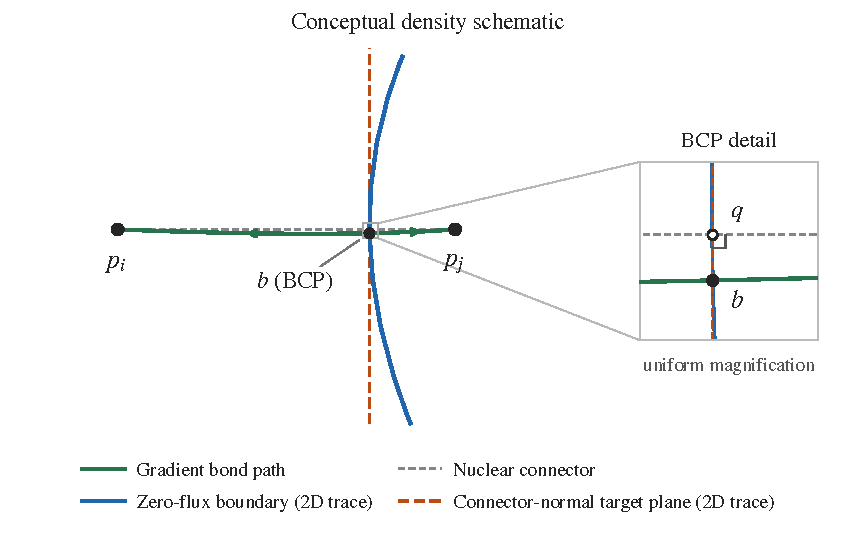
\includegraphics[width=\linewidth]{figures/figure_E_bcp_projection.pdf}
\caption{A conceptual density model in a two-dimensional section. The bond path consists of gradient-ascent branches from the BCP $b$ toward the two atomic attractors. The curved zero-flux boundary passes through $b$ and bends around the right-hand basin. The connector-normal target plane contains both $b$ and its projection $q$; the inset resolves their small separation. Passing through $b$ does not require agreement with the boundary's tangent or curvature. The geometry is illustrative, not taken from a benchmark molecule, and the plane trace does not assert a finite realized power face.}
\label{fig:bcp-projection}
\end{figure}

For fitted weights $\widehat w$, the pairwise plane $H_{ij}(\widehat w)$ has the same normal but may have a different offset. Its distance from the original BCP is exactly
\begin{equation}
 \operatorname{dist}\bigl(b,H_{ij}(\widehat w)\bigr)
 =d_{ij}\bigl|t_{ij}(\widehat w)-t_{ij}^{\mathrm{BCP}}\bigr|.
 \label{eq:bcp-plane-distance}
\end{equation}
Equation~\eqref{eq:bcp-plane-distance} explains the length error used for the fitted models. It concerns the infinite pairwise plane. Even zero distance does not place $b$ on the actual shared face: the other atoms may dominate the power distance there, as in the general distinction of Section~\ref{subsec:faces}.

Nor does a plane through one boundary point necessarily approximate the whole boundary well. Its normal is constrained by the nuclear connector, while the physical boundary can have a different tangent plane and nonzero curvature (Figure~\ref{fig:bcp-projection}). The boundary's intersection with the connector need not be $q$. A best plane approximation to a surface patch would require a choice of patch and error criterion, which is not part of these experiments. In addition, offsets from different BCPs can violate the cycle compatibility condition of Section~3. These are separate limitations of the chosen geometric family and the available observations.

\FloatBarrier
\subsection{Dataset, predictors and error aggregation}
\label{app:molecular-protocols}

The J1 benchmark contains 100 neutral singlet molecules, with 50 acyclic and 50 cyclic structures containing H, C, N, O, F, S and Cl. The dataset was assembled through deterministic PubChem searches \cite{PubChem2025}, followed by RDKit filtering and deduplication by molecular connectivity \cite{RDKit2026}. The selection records and final molecule manifest are in \path{data/qtaim_main/} of the frozen archive \cite{PowerfitArchive2026}. Its \path{scripts/qtaim/README.md} describes the calculation pipeline, and \path{results/qtaim_main/README.md} locates the J1--J4 result records.

Geometry optimization used geomeTRIC \cite{WangSong2016} with PySCF energies and gradients; the subsequent single-point calculations also used PySCF \cite{Sun2020}. Both used the B3LYP functional \cite{Becke1993,Stephens1994} and def2-SVP basis \cite{WeigendAhlrichs2005}. Multiwfn supplies the critical points and their reported atom-pair associations \cite{LuChen2012,Lu2024Multiwfn}; the reference graph uses those associations, deduplicated as unordered pairs. A separate explicit-hydrogen RDKit graph supplies the bonded label: two atoms are bonded precisely when their graph distance is one. Thus both bonded and nonbonded reference pairs can have a BCP.

The archive's reproduction environment is specified in
\texttt{environments/\allowbreak requirements-lock-py313.txt}.
It includes PySCF 2.12.1, geomeTRIC 1.1 and RDKit 2026.3.1.

J1 also records the BCP distance from the nuclear connector. A distance at most $0.02$~\AA{} occurs for 3,637 of the 3,703 bonded reference pairs ($98.22\%$), but only 3 of the 272 nonbonded pairs ($1.10\%$). This describes the landmarks' spatial distribution; by Eq.~\eqref{eq:bcp-projection}, off-axis displacement alone does not create a separator-offset error.

The proatomic inputs are spherically averaged radial electron-density profiles of isolated neutral ground-state atoms, computed with PySCF at B3LYP/def2-SVP and exported through Multiwfn. For unlike atoms separated by $d$, a bounded scalar minimization locates a minimum of
\[
 \rho_i(x)+\rho_j(d-x),\qquad 0\le x\le d.
\]
The radial profiles use piecewise cubic Hermite interpolation. Homonuclear pairs are assigned $x=d/2$. The lookup covers separations from $0.5$ to $5$~\AA{} at $0.01$~\AA{} spacing. At application time, it linearly interpolates the position $x$ and the normalized fraction $t$ separately as functions of $d$. Consequently $x_{\mathrm{lookup}}(d)$ need not equal $d\,t_{\mathrm{lookup}}(d)$ between tabulated distances. The raw proatomic length error uses the former; the fitted model takes the latter as its observations.

For an evaluated subset $S$ of pairs pooled across molecules, the reported length error is
\begin{equation}
 \operatorname{RMSE}_{\!\text{\AA}}(S)
 =\left(\frac{1}{|S|}\sum_{e\in S}\varepsilon_e^2\right)^{1/2},
 \label{eq:molecular-pooled-rmse}
\end{equation}
where $\varepsilon_e=d_e(t_e^{\mathrm{fit}}-t_e^{\mathrm{BCP}})$ for a fitted model and $\varepsilon_e=x_e^{\mathrm{lookup}}-d_e t_e^{\mathrm{BCP}}$ for the raw proatomic prediction. The midpoint error is $\varepsilon_e=d_e(1/2-t_e^{\mathrm{BCP}})$. These are not means of per-molecule RMSE; molecules with more evaluated pairs contribute more terms. J2's direct BCP-target reference fit minimizes the unweighted squared fraction errors separately on each molecule's full reference graph. In length-error notation this objective weights $\varepsilon_e^2$ by $1/d_e^2$, and it does not separately minimize the nonbonded subset error.

\subsection{Candidate graphs and realized pairs}
\label{app:molecular-candidates}

The nonperiodic molecular diagrams use atom-coordinate bounding boxes padded by $5$~\AA{} in the reference calculations. The distance cutoffs selecting J3's input pairs are a separate choice.

A realized pair is counted as \emph{visible} when the connector-line intersection belongs to its clipped face under the archived polygon-membership test \cite{Pyvoro2_063}. This numerical convention includes boundary points rather than requiring a strictly positive analytic gap. In orthonormal face coordinates measured in \AA{}, the test treats oriented edge cross products of magnitude at most $10^{-10}$~\AA$^2$ as zero. The resulting \texttt{intersection\_inside} flag supplies the visibility filter in J3 and the eligible-face selection in J4b.

Table~\ref{tab:molecular-candidates} collects the three cutoff settings. Every setting contains and realizes all 3,975 reference pairs, which are evaluated before visibility filtering. The visible subset retains 3,973 reference pairs in each setting.

\begin{table}[htbp]
\centering
\footnotesize
\setlength{\tabcolsep}{3.5pt}
\caption{J3 candidate-pair sweep. RMSE in \AA{} pools errors on all 3,975 realized reference pairs before visibility filtering. Precision and recall compare all connector-visible realized pairs, under the clipped-face convention in the text, with the fixed reference set. Counts of realized and visible pairs cover the whole diagram, including pairs outside the fitted candidates.}
\label{tab:molecular-candidates}
\begin{tabular}{@{}lrrrrrr@{}}
\toprule
\shortstack{Cutoff\\(\AA)} & Candidates & Realized & Visible & RMSE & \shortstack{Visible\\precision} & \shortstack{Visible\\recall} \\
\midrule
4.0 & 27,178 & 19,472 & 5,704 & 0.0746 & 0.6965 & 0.9995 \\
4.5 & 32,991 & 19,463 & 5,700 & 0.0770 & 0.6970 & 0.9995 \\
5.0 & 39,054 & 19,468 & 5,703 & 0.0786 & 0.6967 & 0.9995 \\
\bottomrule
\end{tabular}
\end{table}

Pairs outside the candidate set account for 2,360, 1,660 and 1,059 of the realized pairs at cutoffs $4$, $4.5$ and $5$~\AA{}, respectively; after visibility filtering, the corresponding counts are 21, 3 and 0. These counts illustrate why a score restricted to input pairs can differ from J3's whole-diagram pair evaluation. Visibility is a post hoc filter here and does not trigger a new fit.

\subsection{Local diagnostics and limits of the auxiliary checks}
\label{app:molecular-diagnostics}

J4a compares the analytic formulas with diagnostics computed from the tessellation in the reference box. The visibility decisions agree on all 38,746 recorded faces. On the 11,677 visible faces, the maximum clipped-clearance discrepancy is $3.52\times10^{-15}$~\AA{}. The population consists of faces already reported by the tessellation; this check does not test detection of missing faces.

For J4b, eligible faces are realized, connector-visible under the convention of \ref{app:molecular-candidates}, and nonbonded under the RDKit convention. Faces from all molecules are pooled separately for the ordinary Voronoi model and the J3 power fit at the $5$~\AA{} cutoff. The ranked clearance is $c_{ij}^{\Omega}$ from Eq.~\eqref{eq:clipped-clearance}; both clearance and face area refer to the clipped reference-box diagrams. Each population is ranked by decreasing clearance, decreasing face area, or increasing pair distance. Writing $y_k\in\{0,1\}$ for the QTAIM-reference label at rank $k$ and $N_+=\sum_k y_k$, the archived average precision is
\[
 \operatorname{AP}
 =\frac{1}{N_+}\sum_k y_k\,
   \frac{\sum_{\ell\le k}y_\ell}{k}.
\]
It is the mean precision at the ranks occupied by positive reference pairs. The archived stable sort preserves record order for equal scores. This calculation is performed once on each pooled population, rather than averaging molecule-level AP values. The exploratory clearance cutoff of $0.50$~\AA{} in the source archive is not a calibrated classification rule.

The additional J4c molecular illustrations use fits to projected BCP targets, not J3's proatomic candidate observations. They are therefore not used here as evidence for that prediction pipeline. J4d varies box margins over $3$, $5$, $7$ and $10$~\AA{}. Voronoi geometries are recomputed, giving 18,798, 19,278, 19,605 and 19,830 realized-pair records. In contrast, all 19,468 recovered-powerfit records are reused unchanged at each margin. These repetitions do not independently establish robustness of the recovered-powerfit geometry to a changed clipping box.

% Sources: frozen powerfit-80933a1 archive, data/qtaim_main and results/qtaim_main.
% BCP associations: scripts/qtaim/run_multiwfn_topology.py, parse_multiwfn_output.
% Proatomic predictor: scripts/qtaim/_proatomic_pairlaw.py and data/proatomic/.
% J2/J3 pooling: analyze_qtaim_true_support_ladder.py / analyze_qtaim_candidate_recovery.py.
% AP definition: scripts/build_manuscript_tables.py, _average_precision and
% table_j4_clearance_ranking; the tie convention is retained from that source.
% Figure E is a deliberately chosen geometric schematic, not molecular data.


\end{document}
